% Edit only the text between matching begin and end lines.
\documentclass[11pt,a4paper]{article}
% Shared preamble for TMUA worked solutions. Local edits here are overwritten.

% Reproducible PDFs: no timestamps, no trailer id, no build-path details.
\ifdefined\pdfsuppressptexinfo
  \pdfsuppressptexinfo=-1
  \pdfinfoomitdate=1
  \pdftrailerid{}
\fi

\usepackage{graphicx}
\usepackage{mathtools}
\usepackage{amssymb}
\usepackage{amsmath}
\usepackage{amsthm}
\usepackage{enumitem}
\usepackage{microtype}
\usepackage[table]{xcolor}
\usepackage{array}
\usepackage{booktabs}
\usepackage{tabularx}
\usepackage{longtable}
\usepackage{ragged2e}
\usepackage{fancyhdr}
\usepackage{etoolbox}
\usepackage[
  a4paper,
  left=0.8in,
  right=1in,
  top=1in,
  bottom=0.5in,
  headheight=14pt,
  headsep=0.4in
]{geometry}

\usepackage{pgfplots}
\pgfplotsset{compat=1.18}
\usepgfplotslibrary{fillbetween, polar}
\usetikzlibrary{calc, positioning}
\usetikzlibrary{angles, quotes}
\usetikzlibrary{arrows.meta}
\usetikzlibrary{decorations.pathreplacing, decorations.markings}
\usetikzlibrary{patterns}
\usetikzlibrary{intersections}

\usepackage{tocloft}
\usepackage[hidelinks]{hyperref}
\hypersetup{pdfauthor={danieljsmith.org}, pdfcreator={}, pdfsubject={}, pdfkeywords={}}
\urlstyle{same}
\tocloftpagestyle{djssolutions}
\setlength{\cftbeforesubsecskip}{2pt}
\setlength{\cftsubsecindent}{1.5em}
\setlength{\cftsubsecnumwidth}{0pt}
\renewcommand{\cftsubsecfont}{\small\color{black}}
\renewcommand{\cftsubsecpagefont}{\small\color{black}}
\renewcommand{\cftsubsecleader}{\hfill}

% `most` carries the breakable and enhanced libraries the solution box needs.
\usepackage[most]{tcolorbox}
\definecolor{scarlet}{RGB}{205, 40, 75}

\setlength{\parindent}{0pt}

% \djsSolutionsSetup{<paper title>}, called once after this file.
\newcommand{\djsSolnPaperTitle}{}
\newcommand{\djsSolutionsSetup}[1]{%
  \hypersetup{pdftitle={#1 Solutions}}%
  \renewcommand{\djsSolnPaperTitle}{#1}}

% \djsTitleSetup{<booklet>}{<title>}{<paper name>}{<questions>}{<minutes>},
% called once after the setup line, sets the title block that opens the
% contents page, as on the question paper: TMUA and the booklet in spaced
% burgundy capitals, the title, a hairline led by the solution box's short
% scarlet rule, then the paper's name with the question count and, when
% given, the time allowed. Its colours are the site's accent, rule and muted
% text colours.
\definecolor{djsBurgundy}{RGB}{118, 59, 67}
\definecolor{djsHairline}{RGB}{216, 213, 205}
\definecolor{djsSlash}{RGB}{170, 166, 158}
\definecolor{djsMuted}{RGB}{96, 101, 106}
\makeatletter
\newcommand{\djs@booklet}{}
\newcommand{\djs@title}{}
\newcommand{\djs@papername}{}
\newcommand{\djs@details}{}
\newcommand{\djs@caps}[1]{\textls[180]{\MakeUppercase{#1}}}
\newcommand{\djs@dot}{\hspace{0.45em}\textperiodcentered\hspace{0.45em}}
\newcommand{\djsTitleSetup}[5]{%
  \renewcommand{\djs@booklet}{#1}%
  \renewcommand{\djs@title}{#2}%
  \renewcommand{\djs@papername}{#3}%
  \renewcommand{\djs@details}{%
    #4~question\ifnum#4=1 \else s\fi
    \ifblank{#5}{}{\djs@dot#5~minutes}}}
\newcommand{\djsContentsTitle}{%
  {\raggedright\color{djsBurgundy}\footnotesize\bfseries
    \djs@caps{TMUA}{\color{djsSlash}\hspace{0.55em}/\hspace{0.55em}}%
    \djs@caps{\djs@booklet}\par}%
  \vspace{7pt}%
  {\raggedright\fontsize{24.88}{28}\selectfont\djs@title\par}%
  \vspace{9pt}%
  \noindent\makebox[0pt][l]{\color{djsHairline}\rule[0.9pt]{\linewidth}{0.6pt}}%
  {\color{scarlet}\rule{3.5cm}{2.2pt}}\par
  \vspace{5pt}%
  {\small\color{djsMuted}\djs@papername\hfill\djs@details\par}%
  \vspace{8pt}}
\makeatother

% The header appears only on the contents page and each question's opening
% page. Continuation pages use the empty default style.
\fancypagestyle{djssolutions}{%
  \fancyhead{}%
  \fancyfoot{}%
  \renewcommand{\headrulewidth}{0.9pt}%
  \fancyhead[L]{\textit{Solutions} - \djsSolnPaperTitle}%
  \fancyhead[R]{\href{https://danieljsmith.org/?utm_source=pdf&utm_campaign=tmua&utm_content=solutions}{danieljsmith.org}}%
}
\pagestyle{empty}

% \djsLastUpdated{<date>}, called once after the setup line: one line
% at the foot of the first page only, left-aligned under the left header at
% the 0.8in left margin. It is drawn over the page rather than set as a
% footer, so no page style changes.
\newcommand{\djsLastUpdated}[1]{%
  \AtBeginDocument{\AddToHookNext{shipout/foreground}{%
    \put(0.8in,-\dimexpr\paperheight-0.32in\relax){\makebox[0pt][l]{%
      \footnotesize Last updated #1}}}}}

\newcolumntype{Y}{>{\RaggedRight\arraybackslash}X}

% Question layout, identical to the question paper's.
\newcommand{\djsTocTopic}[1]{%
  \ifblank{#1}{}{%
    \texorpdfstring
      {\hspace{0.9em}{\footnotesize\itshape\color{black!45}#1}}
      { \textendash\ #1}}}
\newcommand{\djsTopicLine}[1]{%
  \ifblank{#1}{}{%
    {\raggedleft\footnotesize\itshape\color{black!45}#1\par}%
    \vspace{-0.6\baselineskip}}}
\newcommand{\questionitem}[1][]{%
  \item\phantomsection
  \addcontentsline{toc}{subsection}{%
    Question \number\value{enumi}\protect\djsTocTopic{#1}}%
}
\renewcommand{\contentsname}{Questions}
\newcommand{\djsFrontMatter}{%
  \vspace*{6pt}%
  \djsContentsTitle
  \vspace{14pt}%
  \tableofcontents
  \newpage
}

% The solution body: a white breakable box with a left scarlet rule. The
% rule continues onto a continuation page and stops where the solution
% stops, then turns into a short horizontal of the same weight so the
% solution visibly ends. The argument is the answer label.
\newcommand{\djsSolutionAnswer}[1]{%
  {\color{scarlet}\bfseries Answer\ \ #1}}
\newtcolorbox{djsSolution}[1]{%
  enhanced, breakable, frame hidden, sharp corners, colback=white,
  height fixed for=first and middle, height fill,
  extras unbroken and last={natural height},
  borderline west={2.2pt}{0pt}{scarlet},
  left=11pt, right=0pt, top=5pt, bottom=13pt,
  before skip=13pt, after skip=4pt,
  overlay unbroken and last={%
    \fill[scarlet] (frame.south west)
      rectangle ([xshift=3.5cm, yshift=2.2pt]frame.south west);},
  before upper={\setlength{\parskip}{6pt}%
                {\color{scarlet}\bfseries Solution}%
                \hfill\djsSolutionAnswer{#1}\par\vspace{4pt}}}

% Solution figures sit inside the box and are drawn smaller than question
% figures; \scalebox shrinks node text with the drawing.
\newcommand{\SolnFigureScale}{0.85}
\newsavebox{\djsSolnFigureBox}
\newenvironment{djsSolutionFigure}
  {\par\vspace{4pt}\begin{center}\begin{lrbox}{\djsSolnFigureBox}}
  {\end{lrbox}\scalebox{\SolnFigureScale}{\usebox{\djsSolnFigureBox}}%
   \end{center}\vspace{2pt}\par}

\djsSolutionsSetup{TMUA Set C Paper 1}
\djsLastUpdated{3 October 2026}
\begin{document}
\thispagestyle{djssolutions}
\djsFrontMatter
\clearpage
\thispagestyle{djssolutions}
\vspace*{8pt}
\djsTopicLine{Inequalities}
\begin{enumerate}[label=\textbf{\arabic*.},leftmargin=*,itemsep=0pt,start=1]
\questionitem[Inequalities]
% begin q000771 stem
For which real values of $x$ is the following inequality true?
\[
x^2<(x-3)^2<(2x+1)^2
\]
% end q000771 stem

\par\vspace*{12pt}
\begin{tabularx}{\linewidth}{@{}>{\bfseries}l Y@{}}
A &
% begin q000771 choice A
$x<-4$ or $\dfrac{2}{3}<x<\dfrac{3}{2}$
% end q000771 choice A
\\[0.8em]
B &
% begin q000771 choice B
$x<-4$ or $x>\dfrac{2}{3}$
% end q000771 choice B
\\[0.8em]
C &
% begin q000771 choice C
$-4<x<\dfrac{2}{3}$
% end q000771 choice C
\\[0.8em]
D &
% begin q000771 choice D
$-4<x<\dfrac{3}{2}$
% end q000771 choice D
\\[0.8em]
E &
% begin q000771 choice E
$\dfrac{2}{3}<x<\dfrac{3}{2}$ or $x>4$
% end q000771 choice E
\\
\end{tabularx}

\begin{djsSolution}{A}
% begin q000771 solution
The chain is true only when both inequalities hold:
\[
\begin{aligned}
x^2&<(x-3)^2\\[5pt]
(x-3)^2&<(2x+1)^2
\end{aligned}
\]

First solve the left-hand inequality. Expanding and simplifying,
\[
x^2<x^2-6x+9
\implies 6x<9
\implies x<\frac32
\]

Now solve the second inequality. Rearranging,
\[
(2x+1)^2-(x-3)^2>0
\]

Using the difference-of-two-squares identity $a^2-b^2=(a-b)(a+b)$,
\[
\begin{aligned}
\bigl[(2x+1)-(x-3)\bigr]\bigl[(2x+1)+(x-3)\bigr]&>0\\[5pt]
(x+4)(3x-2)&>0
\end{aligned}
\]
Using difference-of-two-squares here is optional: expanding the squared expressions and then factorising gives the same result.

A product is positive when its factors are both positive or both negative. For both factors to be positive,
\[
x>-4\quad\text{and}\quad x>\frac23
\implies x>\frac23
\]

For both factors to be negative,
\[
x<-4\quad\text{and}\quad x<\frac23
\implies x<-4
\]

Thus the second inequality holds when
\[
x<-4\quad\text{or}\quad x>\frac23
\]

Finally, take the overlap with $x<\frac32$. On the aligned number lines below, blue shows the first inequality, orange the second, and pink their overlap. The marked values are not drawn to scale.

\begin{djsSolutionFigure}
% begin q000771 figure F1
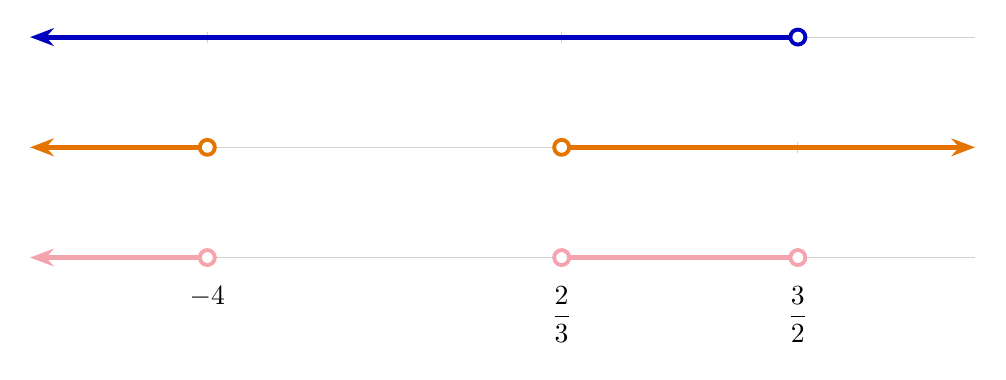
\begin{tikzpicture}[x=1.5cm,y=1.4cm]
\def\leftbound{-1.5}
\def\rightbound{6.5}
\def\firstcritical{0}
\def\secondcritical{3}
\def\thirdcritical{5}
\colorlet{solutionblue}{blue!75!black}
\colorlet{solutionorange}{orange!90!black}
\colorlet{solutionpurple}{pink!85!purple}

\foreach \row in {0,1,2} {
  \coordinate (L\row) at (\leftbound,\row);
  \coordinate (R\row) at (\rightbound,\row);
  \coordinate (A\row) at (\firstcritical,\row);
  \coordinate (B\row) at (\secondcritical,\row);
  \coordinate (C\row) at (\thirdcritical,\row);
  \draw[gray!35,line width=0.4pt] (L\row) -- (R\row);
}

\foreach \point in {A2,B2,C1} {
  \draw[gray!35,line width=0.4pt]
    ([yshift=-0.07cm]\point) -- ([yshift=0.07cm]\point);
}

\draw[solutionblue,line width=1.8pt,-{Stealth[length=3mm]}]
  (C2) -- (L2);
\draw[solutionorange,line width=1.8pt,-{Stealth[length=3mm]}]
  (A1) -- (L1);
\draw[solutionorange,line width=1.8pt,-{Stealth[length=3mm]}]
  (B1) -- (R1);
\draw[solutionpurple,line width=1.8pt,-{Stealth[length=3mm]}]
  (A0) -- (L0);
\draw[solutionpurple,line width=1.8pt] (B0) -- (C0);

\foreach \point/\rowcolour in {C2/solutionblue,A1/solutionorange,B1/solutionorange,A0/solutionpurple,B0/solutionpurple,C0/solutionpurple} {
  \draw[draw=\rowcolour,fill=white,line width=1.4pt]
    (\point) circle[radius=2.7pt];
}

\node[below=7pt] at (A0) {$-4$};
\node[below=7pt] at (B0) {$\dfrac23$};
\node[below=7pt] at (C0) {$\dfrac32$};
\end{tikzpicture}
% end q000771 figure F1
\end{djsSolutionFigure}

The overlap is
\[
\boxed{x<-4\quad\text{or}\quad \frac23<x<\frac32}
\]

All endpoints remain excluded because the inequalities are strict. The correct option is \textbf{A}.\\[5pt]

\textit{Alternative Solution:}

Test values that distinguish the proposed sets: $0$ lies in the central ranges, $2$ tests the upper ranges, and $-5$ lies below $-4$.

For $x=0$, the original chain evaluates to
\[
0<9<1
\]
This is false. Options C and D both include $0$, so eliminate them.

For $x=2$, the original chain evaluates to
\[
4<1<25
\]
This is false. Option B includes $2$ because $2>\frac23$, so eliminate B.

For $x=-5$, the original chain evaluates to
\[
25<64<81
\]
This is true. Of the remaining options, A includes $-5$, whereas E does not, so eliminate E.

The correct option is therefore \textbf{A}, as it is the only one remaining.
% end q000771 solution
\end{djsSolution}
\end{enumerate}
\clearpage
\thispagestyle{djssolutions}
\vspace*{8pt}
\djsTopicLine{Geometry}
\begin{enumerate}[label=\textbf{\arabic*.},leftmargin=*,itemsep=0pt,start=2]
\questionitem[Geometry]
% begin q000659 stem
$ABCD$ is a rectangle with $AB=3\text{ cm}$ and $AD=10\text{ cm}$. 

Point $E$ lies on $BC$, and $\angle AED=90^\circ$

What is the value of $BE\times EC$?
% end q000659 stem

\begin{center}
% begin q000659 diagram
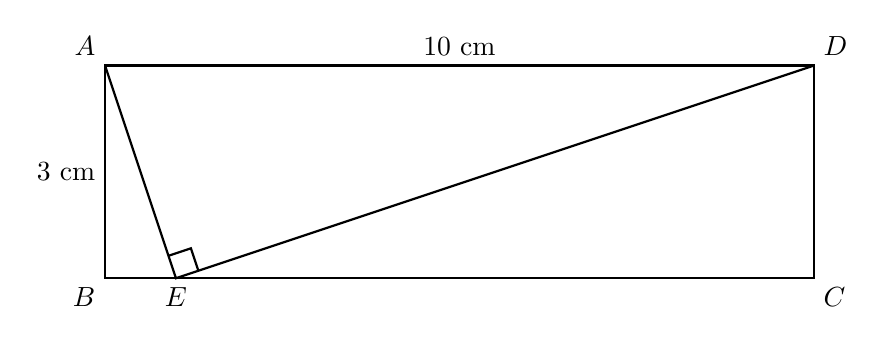
\begin{tikzpicture}[x=0.9cm,y=0.9cm]
\def\rectwidth{10}
\def\rectheight{3}
\def\BE{1}

\coordinate (B) at (0,0);
\coordinate (A) at (0,\rectheight);
\coordinate (C) at (\rectwidth,0);
\coordinate (D) at (\rectwidth,\rectheight);
\coordinate (E) at (\BE,0);

\draw[thick, black] (A) -- (B) -- (C) -- (D) -- cycle;
\draw[thick, black] (A) -- (E) -- (D);

\pic[draw, thick, angle radius=3mm] {right angle=D--E--A};

\node[above left] at (A) {$A$};
\node[below left] at (B) {$B$};
\node[below right] at (C) {$C$};
\node[above right] at (D) {$D$};
\node[below] at (E) {$E$};

\path (A) -- (B) node[midway, left] {$3\text{ cm}$};
\path (A) -- (D) node[midway, above] {$10\text{ cm}$};
\end{tikzpicture}
% end q000659 diagram
\end{center}

\par\vspace*{12pt}
\begin{tabularx}{\linewidth}{@{}>{\bfseries}l Y@{}}
A &
% begin q000659 choice A
$9\text{ cm}^2$
% end q000659 choice A
\\[0.8em]
B &
% begin q000659 choice B
$18\text{ cm}^2$
% end q000659 choice B
\\[0.8em]
C &
% begin q000659 choice C
$41\text{ cm}^2$
% end q000659 choice C
\\[0.8em]
D &
% begin q000659 choice D
$50\text{ cm}^2$
% end q000659 choice D
\\[0.8em]
E &
% begin q000659 choice E
$82\text{ cm}^2$
% end q000659 choice E
\\
\end{tabularx}

\begin{djsSolution}{A}
% begin q000659 solution
Measure lengths in centimetres and write $BE=x$. Since opposite sides of a rectangle are equal, $BC=AD=10$ and $CD=AB=3$, so $EC=10-x$.

Applying Pythagoras' theorem in $ABE$ and $ECD$ gives
\[
\begin{aligned}
AE^2&=AB^2+BE^2=3^2+x^2=x^2+9\\[5pt]
DE^2&=CD^2+EC^2=3^2+(10-x)^2=(10-x)^2+9
\end{aligned}
\]

Taking positive square roots gives the lengths labelled below.

\begin{djsSolutionFigure}
% begin q000659 figure F1
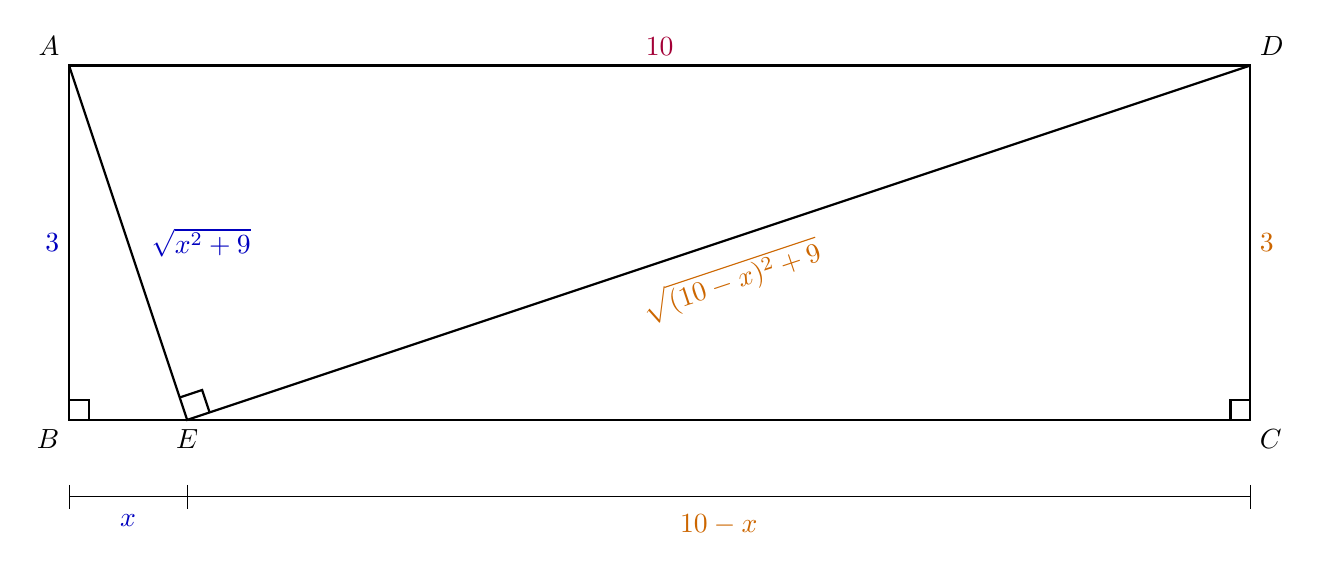
\begin{tikzpicture}[x=1.5cm,y=1.5cm]
\def\rectwidth{10}
\def\rectheight{3}
\def\BE{1}
\colorlet{solutionblue}{blue!75!black}
\colorlet{solutionorange}{orange!80!black}
\colorlet{solutionpurple}{purple!85!black}

\coordinate (B) at (0,0);
\coordinate (A) at (0,\rectheight);
\coordinate (C) at (\rectwidth,0);
\coordinate (D) at (\rectwidth,\rectheight);
\coordinate (E) at (\BE,0);

\draw[thick, black] (A) -- (B) -- (C) -- (D) -- cycle;
\draw[thick, black] (A) -- (E) -- (D);

\pic[draw, thick, angle radius=3mm] {right angle=D--E--A};
\pic[draw, thick, angle radius=2.5mm] {right angle=E--B--A};
\pic[draw, thick, angle radius=2.5mm] {right angle=D--C--E};

\node[above left] at (A) {$A$};
\node[below left] at (B) {$B$};
\node[below right] at (C) {$C$};
\node[above right] at (D) {$D$};
\node[below] at (E) {$E$};

\path (A) -- (B)
  node[midway, left, text=solutionblue] {$3$};
\path (A) -- (D)
  node[midway, above, text=solutionpurple] {$10$};
\path (C) -- (D)
  node[midway, right, text=solutionorange] {$3$};
\path (A) -- (E)
  node[midway, right=5pt, text=solutionblue] {$\sqrt{x^2+9}$};
\path (E) -- (D)
  node[midway, sloped, below=5pt, text=solutionorange]
  {$\sqrt{(10-x)^2+9}$};

\draw[thin, black] (0,-0.65) -- (1,-0.65)
  node[midway, below=3pt, text=solutionblue] {$x$};
\draw[thin, black] (1,-0.65) -- (10,-0.65)
  node[midway, below=3pt, text=solutionorange] {$10-x$};
\foreach \position in {0,1,10} {
  \draw[thin, black] (\position,-0.55) -- (\position,-0.75);
}
\end{tikzpicture}
% end q000659 figure F1
\end{djsSolutionFigure}

Now apply Pythagoras' theorem in $AED$, where $AD$ is the hypotenuse:
\[
AD^2=AE^2+DE^2
\implies 10^2=(x^2+9)+\bigl((10-x)^2+9\bigr)
\]

Expanding and collecting terms,
\[
\begin{aligned}
100&=x^2+9+100-20x+x^2+9\\[5pt]
&=2x^2-20x+118
\end{aligned}
\]

Rearranging and dividing by $2$,
\[
x^2-10x+9=0
\]

Factorising,
\[
(x-1)(x-9)=0
\implies x=1\,\,\text{or}\,\, x=9
\]

Both values place $E$ on $BC$. The required product is $x(10-x)$, so either value gives the same result
\[
BE\times EC=1\times9=\boxed{9\text{ cm}^2}
\]
so the correct option is \textbf{A}.

There is also a shorter finish: the quadratic equation gives the product without finding $x$:
\[
x^2-10x+9=0
\implies 10x-x^2=9
\implies x(10-x)=9
\]

This is exactly $BE\times EC$\\[5pt]

\textit{Alternative Solution:} (Similar triangles)

We can obtain the product directly by showing that the two smaller right-angled triangles are similar. Write $\theta=\angle BAE$. We will show that $\angle DEC=\theta$ too, as marked below.

\begin{djsSolutionFigure}
% begin q000659 figure F2
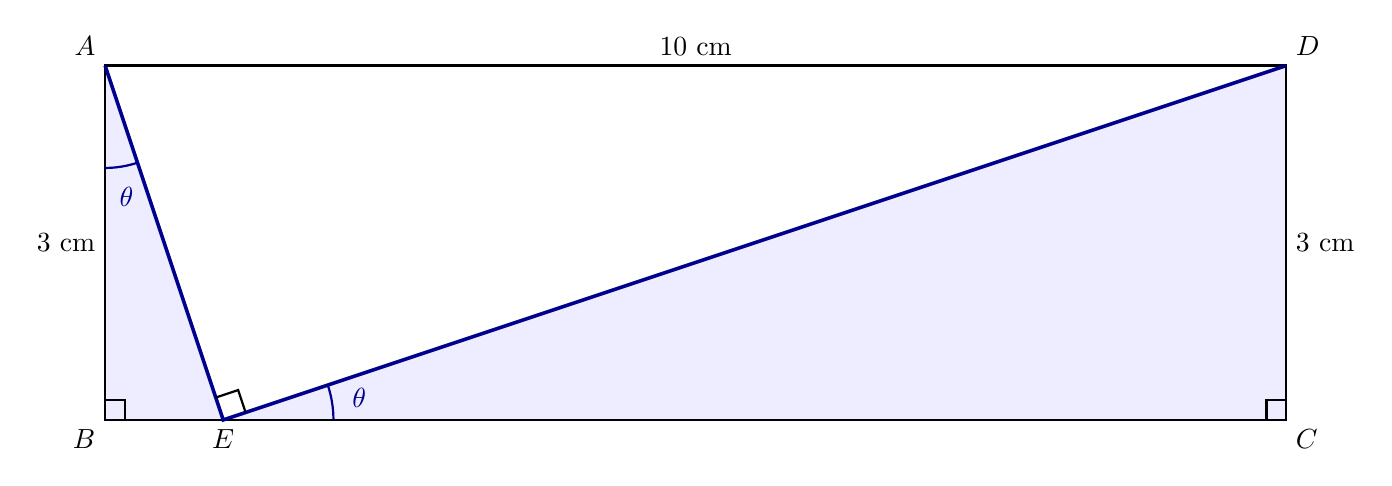
\begin{tikzpicture}[x=1.5cm,y=1.5cm]
\def\rectwidth{10}
\def\rectheight{3}
\def\BE{1}

\coordinate (B) at (0,0);
\coordinate (A) at (0,\rectheight);
\coordinate (C) at (\rectwidth,0);
\coordinate (D) at (\rectwidth,\rectheight);
\coordinate (E) at (\BE,0);

\fill[blue!7] (A) -- (B) -- (E) -- cycle;
\fill[blue!7] (E) -- (C) -- (D) -- cycle;

\draw[thick, black] (A) -- (B) -- (C) -- (D) -- cycle;
\draw[line width=1.3pt, blue!55!black] (A) -- (E) -- (D);

\pic[draw, thick, angle radius=3mm] {right angle=D--E--A};
\pic[draw, thick, angle radius=2.5mm] {right angle=E--B--A};
\pic[draw, thick, angle radius=2.5mm] {right angle=D--C--E};

\pic["$\theta$", draw=blue!55!black, text=blue!55!black,
      thick, angle radius=13mm, angle eccentricity=1.3]
      {angle=B--A--E};
\pic["$\theta$", draw=blue!55!black, text=blue!55!black,
      thick, angle radius=14mm, angle eccentricity=1.25]
      {angle=C--E--D};

\node[above left] at (A) {$A$};
\node[below left] at (B) {$B$};
\node[below right] at (C) {$C$};
\node[above right] at (D) {$D$};
\node[below] at (E) {$E$};

\path (A) -- (B) node[midway, left] {$3\text{ cm}$};
\path (A) -- (D) node[midway, above] {$10\text{ cm}$};
\path (C) -- (D) node[midway, right] {$3\text{ cm}$};
\end{tikzpicture}
% end q000659 figure F2
\end{djsSolutionFigure}

Since $\angle ABE=90^\circ$, the angle sum in triangle $ABE$ gives
\[
\angle AEB=180^\circ-90^\circ-\theta=90^\circ-\theta
\]

At $E$, the angles $AEB$, $AED$ and $DEC$ lie along the straight line $BC$, so they sum to $180^\circ$. Using $\angle AED=90^\circ$,
\[
\angle DEC=180^\circ-90^\circ-(90^\circ-\theta)=\theta
\]

Thus triangles $ABE$ and $ECD$ are similar: both have a right angle, and $\angle BAE=\angle DEC$. The corresponding vertices are $A$ and $E$, $B$ and $C$, then $E$ and $D$.

Corresponding sides are in the same ratio. Since $AB$ corresponds to $EC$, and $BE$ to $CD$,
\[
\frac{AB}{EC}=\frac{BE}{CD}
\implies \frac{3}{EC}=\frac{BE}{3}
\]

Multiplying by $3EC$, which is positive,
\[
BE\times EC=9\text{ cm}^2
\]

Again obtaining option \textbf{A}.
% end q000659 solution
\end{djsSolution}
\end{enumerate}
\clearpage
\thispagestyle{djssolutions}
\vspace*{8pt}
\djsTopicLine{Exponentials \& Logarithms}
\begin{enumerate}[label=\textbf{\arabic*.},leftmargin=*,itemsep=0pt,start=3]
\questionitem[Exponentials \& Logarithms]
% begin q000731 stem
For $1<x<81$, the equation
\[\log_2(\log_3 x)+\log_2\!\left(\log_3\frac{81}{x}\right)=1\]

has two solutions. What is the smaller solution?
% end q000731 stem

\par\vspace*{12pt}
\begin{tabularx}{\linewidth}{@{}>{\bfseries}l Y@{}}
A &
% begin q000731 choice A
$3^{2-\sqrt{3}}$
% end q000731 choice A
\\[0.8em]
B &
% begin q000731 choice B
$3^{2-\sqrt{2}}$
% end q000731 choice B
\\[0.8em]
C &
% begin q000731 choice C
$3^{\sqrt{2}}$
% end q000731 choice C
\\[0.8em]
D &
% begin q000731 choice D
$3^{4-\sqrt{2}}$
% end q000731 choice D
\\[0.8em]
E &
% begin q000731 choice E
$3^{2+\sqrt{2}}$
% end q000731 choice E
\\
\end{tabularx}

\begin{djsSolution}{B}
% begin q000731 solution
Both inner logarithms are positive for $1<x<81$, so the logarithm rules apply.

Combining the two base-$2$ logarithms gives
\[
\log_2\!\left[(\log_3 x)\left(\log_3\frac{81}{x}\right)\right]=1
\]

Since $81=3^4$,
\[
\begin{aligned}
\log_3\frac{81}{x}
&=\log_3 81-\log_3 x\\[5pt]
&=4-\log_3 x
\end{aligned}
\]

Substituting gives
\[
\log_2\,\Bigl[(\log_3 x)(4-\log_3 x)\Bigr]=1
\]

Exponentiating to base $2$ gives
\[
(\log_3 x)(4-\log_3 x)=2
\]

This is a hidden quadratic in $\log_3 x$. Put
\[
u=\log_3 x
\]

Since $\log_3 x$ is increasing, the domain $1<x<81$ becomes
\[
0<u<4
\]

The equation is now
\[
u(4-u)=2
\]

Expanding,
\[
4u-u^2=2
\]

Rearranging,
\[
u^2-4u+2=0
\]

The quadratic formula gives
\[
\begin{aligned}
u&=\frac{4\pm\sqrt{(-4)^2-4(1)(2)}}{2(1)}\\[8pt]
&=\frac{4\pm\sqrt{8}}{2}\\[8pt]
&=\frac{4\pm2\sqrt{2}}{2}
\end{aligned}
\]

Hence
\[
u=2-\sqrt{2}\quad\text{or}\quad u=2+\sqrt{2}
\]

Both values lie in the required domain, because $0<\sqrt{2}<2$ gives
\[
0<2-\sqrt{2}<2+\sqrt{2}<4
\]

Since $\log_3 x$ is increasing, the smaller value of $u$ corresponds to the smaller value of $x$. Using $x=3^u$, the smaller solution is
\[
x=3^{2-\sqrt{2}}
\]

The correct option is \textbf{B}.
% end q000731 solution
\end{djsSolution}
\end{enumerate}
\clearpage
\thispagestyle{djssolutions}
\vspace*{8pt}
\djsTopicLine{Trigonometry}
\begin{enumerate}[label=\textbf{\arabic*.},leftmargin=*,itemsep=0pt,start=4]
\questionitem[Trigonometry]
% begin q000750 stem
Triangle $ABC$ is right-angled at $A$, and angle $ABC$ is $30^\circ$

The point $D$ is the midpoint of $AB$

If angle $ACD$ is $\theta$, what is $\cos\theta$?
% end q000750 stem

\begin{center}
% begin q000750 diagram
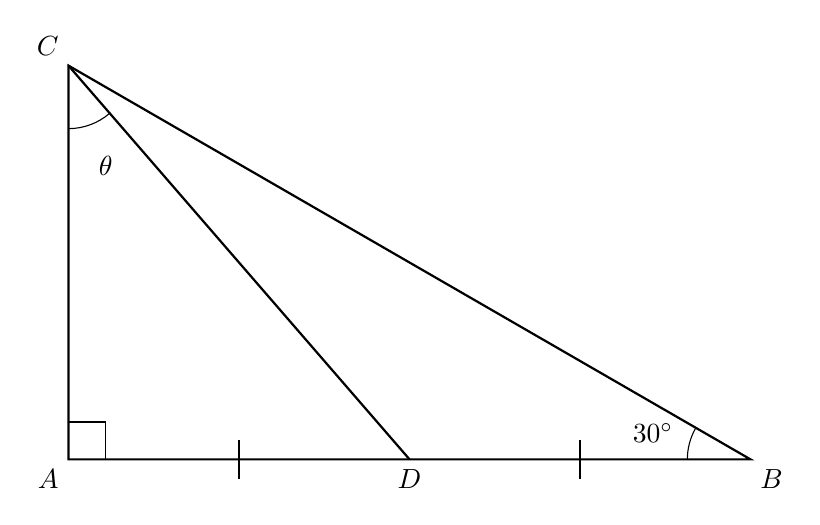
\begin{tikzpicture}[scale=2.5]
\def\height{2}
\pgfmathsetmacro{\base}{sqrt(3)*\height}
\coordinate (A) at (0,0);
\coordinate (B) at (\base,0);
\coordinate (C) at (0,\height);
\coordinate (D) at ($(A)!0.5!(B)$);
\coordinate (TAD) at ($(A)!0.5!(D)$);
\coordinate (TDB) at ($(D)!0.5!(B)$);

\draw[thick,black] (A) -- (B) -- (C) -- cycle;
\draw[thick,black] (C) -- (D);
\draw (A) ++(0.19,0) -- ++(0,0.19) -- ++(-0.19,0);
\foreach \P in {TAD,TDB}{
  \draw[thick] ($ (\P)+(0,-0.10) $) -- ($ (\P)+(0,0.10) $);
}
\pic["$30^\circ$",draw,angle radius=8mm,angle eccentricity=1.6]{angle=C--B--A};
\pic["$\theta$",draw,angle radius=8mm,angle eccentricity=1.7]{angle=A--C--D};

\node[below left] at (A) {$A$};
\node[below right] at (B) {$B$};
\node[above left] at (C) {$C$};
\node[below] at (D) {$D$};
\end{tikzpicture}
% end q000750 diagram
\end{center}

\par\vspace*{12pt}
\begin{tabularx}{\linewidth}{@{}>{\bfseries}l Y@{}}
A &
% begin q000750 choice A
$\dfrac{1}{\sqrt7}$
% end q000750 choice A
\\[0.8em]
B &
% begin q000750 choice B
$\dfrac12$
% end q000750 choice B
\\[0.8em]
C &
% begin q000750 choice C
$\dfrac{\sqrt3}{\sqrt7}$
% end q000750 choice C
\\[0.8em]
D &
% begin q000750 choice D
$\dfrac{2}{\sqrt7}$
% end q000750 choice D
\\[0.8em]
E &
% begin q000750 choice E
$\dfrac{\sqrt3}{2}$
% end q000750 choice E
\\
\end{tabularx}

\begin{djsSolution}{D}
% begin q000750 solution
Let $AD=x$, where $x>0$. Since $D$ is the midpoint of $AB$, we have
$DB=x$
and hence
$
AB=2x
$

First find $AC$ using triangle $ABC$:
\[
\tan30^\circ=\frac{AC}{2x}
\]

Using $\tan30^\circ=1/\sqrt3$,
\[
\frac{AC}{2x}=\frac{1}{\sqrt3}
\]

Therefore
\[
AC=\frac{2x}{\sqrt3}
\]

Now find $CD$ in the right-angled triangle $ACD$. By Pythagoras' theorem,
\[
CD^2=AC^2+AD^2
\]

Substituting,
\[
\begin{aligned}
CD^2&=\left(\frac{2x}{\sqrt3}\right)^2+x^2\\[8pt]
&=\frac{4x^2}{3}+x^2=\frac{7x^2}{3}
\end{aligned}
\]

Since $x>0$ and $CD$ is a length,
\[
CD=\frac{\sqrt7\,x}{\sqrt3}
\]

To complete the side labels on the diagram, use triangle $ABC$:
\[
\sin30^\circ=\frac{AC}{BC}
\]

Rearranging and substituting,
\[
\begin{aligned}
BC&=\frac{AC}{\sin30^\circ}\\[8pt]
&=\frac{2x/\sqrt3}{1/2}=\frac{4x}{\sqrt3}
\end{aligned}
\]

The diagram now shows all the side lengths in terms of $x$.

\begin{djsSolutionFigure}
% begin q000750 figure F1
\begin{tikzpicture}[scale=3.75]
\def\height{2}
\pgfmathsetmacro{\base}{sqrt(3)*\height}
\colorlet{lengthgreen}{green!40!black}
\colorlet{lengthpurple}{violet!85!black}
\colorlet{lengthorange}{orange!80!black}
\coordinate (A) at (0,0);
\coordinate (B) at (\base,0);
\coordinate (C) at (0,\height);
\coordinate (D) at ($(A)!0.5!(B)$);
\coordinate (TAD) at ($(A)!0.5!(D)$);
\coordinate (TDB) at ($(D)!0.5!(B)$);

\draw[thick,black] (A) -- (B) -- (C) -- cycle;
\draw[thick,black] (C) -- (D);
\draw[line width=1.1pt,blue] (A) -- (D) -- (B);
\draw[line width=1.1pt,lengthgreen] (A) -- (C);
\draw[line width=1.1pt,lengthpurple] (C) -- (D);
\draw[line width=1.1pt,lengthorange] (B) -- (C);

\draw (A) ++(0.19,0) -- ++(0,0.19) -- ++(-0.19,0);
\foreach \P in {TAD,TDB}{
  \draw[thick] ($ (\P)+(0,-0.10) $) -- ($ (\P)+(0,0.10) $);
}
\pic["$30^\circ$",draw,angle radius=8mm,angle eccentricity=1.6]{angle=C--B--A};
\pic["$\theta$",draw,angle radius=8mm,angle eccentricity=1.7]{angle=A--C--D};

\node[below left] at (A) {$A$};
\node[below right] at (B) {$B$};
\node[above left] at (C) {$C$};
\node[below] at (D) {$D$};

\path (A) -- (D)
  node[midway,below=4mm,text=blue] {$x$};
\path (D) -- (B)
  node[midway,below=4mm,text=blue] {$x$};
\path (A) -- (C)
  node[midway,left=2mm,text=lengthgreen] {$\dfrac{2x}{\sqrt3}$};
\path (C) -- (D)
  node[midway,sloped,below=2mm,text=lengthpurple]
  {$\dfrac{\sqrt7\,x}{\sqrt3}$};
\path (B) -- (C)
  node[midway,sloped,above=2mm,text=lengthorange]
  {$\dfrac{4x}{\sqrt3}$};
\end{tikzpicture}
% end q000750 figure F1
\end{djsSolutionFigure}

For $\theta$ in triangle $ACD$, the adjacent side is $AC$ and the hypotenuse is $CD$, so
\[
\cos\theta=\frac{AC}{CD}
\]

Substituting and cancelling the non-zero scale factor $x$,
\[
\begin{aligned}
\cos\theta&=\frac{2x/\sqrt3}{\sqrt7\,x/\sqrt3}\\[8pt]
&=\frac{2x}{\sqrt7\,x}= \frac{2}{\sqrt7}
\end{aligned}
\]

The correct option is \textbf{D}.
% end q000750 solution
\end{djsSolution}
\end{enumerate}
\clearpage
\thispagestyle{djssolutions}
\vspace*{8pt}
\djsTopicLine{Sequences \& Series}
\begin{enumerate}[label=\textbf{\arabic*.},leftmargin=*,itemsep=0pt,start=5]
\questionitem[Sequences \& Series]
% begin q000761 stem
An infinite geometric series has positive first term $a$ and common ratio $r$, where $|r| < 1$.
The sum to infinity of this series is $S$.

A second series is formed by taking every third term of the first series, beginning with the first term:
\[ T = u_1 + u_4 + u_7 + u_{10} + \dots \]
where $u_n$ denotes the $n$th term of the first series.\vspace*{3pt}

What is the maximum possible value of $\dfrac{T}{S}$?
% end q000761 stem

\par\vspace*{12pt}
\begin{tabularx}{\linewidth}{@{}>{\bfseries}l Y@{}}
A &
% begin q000761 choice A
$\dfrac{3}{4}$
% end q000761 choice A
\\[0.8em]
B &
% begin q000761 choice B
$1$
% end q000761 choice B
\\[0.8em]
C &
% begin q000761 choice C
$\dfrac{7}{6}$
% end q000761 choice C
\\[0.8em]
D &
% begin q000761 choice D
$\dfrac{4}{3}$
% end q000761 choice D
\\[0.8em]
E &
% begin q000761 choice E
$\dfrac{3}{2}$
% end q000761 choice E
\\[0.8em]
F &
% begin q000761 choice F
$3$
% end q000761 choice F
\\
\end{tabularx}

\begin{djsSolution}{D}
% begin q000761 solution
Write the opening terms of the two series:
\[
\begin{aligned}
S&=a+ar+ar^2+ar^3+\cdots\\[5pt]
T&=a+ar^3+ar^6+ar^9+\cdots
\end{aligned}
\]

Both have first term $a$, but their common ratios are $r$ and $r^3$, respectively. Since $|r|<1$, we also have $|r^3|<1$, so both sums converge.

The geometric sum-to-infinity formula is
\[
\text{Sum to infinity}=\frac{\text{first term}}{1-\text{common ratio}}
\]

Applying it to each series gives
\[
\begin{aligned}
S&=\frac{a}{1-r}\\[8pt]
T&=\frac{a}{1-r^3}
\end{aligned}
\]

Since $a>0$ and $r<1$, we have $S>0$. Forming the ratio gives
\[
\begin{aligned}
\frac{T}{S}
&=\frac{a}{1-r^3}\times\frac{1-r}{a}\\[8pt]
&=\frac{1-r}{1-r^3}
=\frac{r-1}{r^3-1}
\end{aligned}
\]

Since $r^3-1=0$ at $r=1$, the factor theorem tells us that $r-1$ is a factor of the denominator and can be cancelled when $r\ne1$. Polynomial division of $r^3-1$ by $r-1$ gives quotient $r^2+r+1$ with no remainder, so
\[
r^3-1=(r-1)(r^2+r+1)
\]

Alternatively, this follows from the difference of two cubes identity
\[
a^3-b^3=(a-b)(a^2+ab+b^2)
\]
by taking $a=r$ and $b=1$.

As $r\ne1$, cancelling gives
\[
\begin{aligned}
\frac{T}{S}
&=\frac{r-1}{(r-1)(r^2+r+1)}\\[8pt]
&=\frac{1}{r^2+r+1}
\end{aligned}
\]

To maximise a reciprocal with a positive denominator, minimise the denominator: dividing $1$ by a smaller positive number gives a larger value. Complete the square:
\[
\begin{aligned}
r^2+r+1
&=\left(r+\frac12\right)^2-\frac14+1\\[8pt]
&=\left(r+\frac12\right)^2+\frac34
\end{aligned}
\]

The squared term is non-negative, so the denominator is always positive and has minimum value
\[
\frac34
\]

Equality occurs when
\[
r=-\frac12
\]

This value is allowed because
\[
-1<-\frac12<1
\]

Checking this is essential: the minimum over all real values of $r$ must occur within the permitted range for the corresponding maximum to be attainable.

Hence the maximum possible ratio is
\[
\frac{T}{S}=\frac{1}{\frac34}=\frac43
\]

The correct option is \textbf{D}.
% end q000761 solution
\end{djsSolution}
\end{enumerate}
\clearpage
\thispagestyle{djssolutions}
\vspace*{8pt}
\djsTopicLine{Exponentials \& Logarithms}
\begin{enumerate}[label=\textbf{\arabic*.},leftmargin=*,itemsep=0pt,start=6]
\questionitem[Exponentials \& Logarithms]
% begin q000733 stem
Consider the equation
\[
x^{\log_2(x^2)} - 18 x^{\log_2 x} + 32 = 0
\]

What is the sum of all real solutions to this equation?
% end q000733 stem

\par\vspace*{12pt}
\begin{tabularx}{\linewidth}{@{}>{\bfseries}l Y@{}}
A &
% begin q000733 choice A
$1$
% end q000733 choice A
\\[0.8em]
B &
% begin q000733 choice B
$\dfrac{9}{2}$
% end q000733 choice B
\\[0.8em]
C &
% begin q000733 choice C
$6$
% end q000733 choice C
\\[0.8em]
D &
% begin q000733 choice D
$\dfrac{25}{4}$
% end q000733 choice D
\\[0.8em]
E &
% begin q000733 choice E
$\dfrac{13}{2}$
% end q000733 choice E
\\[0.8em]
F &
% begin q000733 choice F
$\dfrac{27}{4}$
% end q000733 choice F
\\[0.8em]
G &
% begin q000733 choice G
$\dfrac{31}{4}$
% end q000733 choice G
\\[0.8em]
H &
% begin q000733 choice H
$18$
% end q000733 choice H
\\
\end{tabularx}

\begin{djsSolution}{F}
% begin q000733 solution
The logarithm $\log_2x$ requires
\[
x>0
\]

For a positive argument, the logarithmic power law is $\log_2(t^k)=k\log_2t$. Applying it here gives
\[
\log_2(x^2)=2\log_2x
\]

Using the index law $a^{2b}=(a^b)^2$, the first term becomes
\[
\begin{aligned}
x^{\log_2(x^2)}&=x^{2\log_2x}\\[5pt]
&=\left(x^{\log_2x}\right)^2
\end{aligned}
\]

To turn the equation into a quadratic, set
\[
u=x^{\log_2x}>0
\]

The original equation is then
\[
u^2-18u+32=0
\]

The numbers $2$ and $16$ have product $32$ and sum $18$, so factorising gives
\[
(u-2)(u-16)=0
\]

Hence
\[
u=2\quad\text{or}\quad u=16
\]

Both values are positive, but these are values of $u$, not the requested values of $x$. We must solve $x^{\log_2x}=u$ for each one.

Taking base-$2$ logarithms and applying the power law gives
\[
\begin{aligned}
\log_2u&=\log_2\left(x^{\log_2x}\right)\\[5pt]
&=(\log_2x)(\log_2x)\\[5pt]
&=(\log_2x)^2
\end{aligned}
\]

By the definition of logarithms, $\log_2x=k$ means $x=2^k$.

For $u=2$, we obtain
\[
(\log_2x)^2=\log_2 2=1
\]

Retaining both square roots gives
\[
\log_2x=1\quad\text{or}\quad\log_2x=-1
\]

Converting back to $x$,
\[
x=2^1=2\quad\text{or}\quad x=2^{-1}=\frac12
\]

For $u=16$, we obtain
\[
(\log_2x)^2=\log_2 16=4
\]

Again retaining both square roots gives
\[
\log_2x=2\quad\text{or}\quad\log_2x=-2
\]

Converting back to $x$,
\[
x=2^2=4\quad\text{or}\quad x=2^{-2}=\frac14
\]

The complete solution set for $x$ is therefore 
\[
\boxed{x = 2,\,\frac12,\,4,\,\frac14}
\]

All four values are positive and distinct. Their sum is
\[
\begin{aligned}
2+\frac12+4+\frac14
&=\frac{8+2+16+1}{4}\\[8pt]
&=\frac{27}{4}
\end{aligned}
\]

The correct option is \textbf{F}.
% end q000733 solution
\end{djsSolution}
\end{enumerate}
\clearpage
\thispagestyle{djssolutions}
\vspace*{8pt}
\djsTopicLine{Differentiation}
\begin{enumerate}[label=\textbf{\arabic*.},leftmargin=*,itemsep=0pt,start=7]
\questionitem[Differentiation]
% begin q000774 stem
A straight line is tangent to both the curve $y=x^2$ and the curve $y=\dfrac{1}{x}$, where $x\ne0$

At what value of $x$ does this line cross the $x$-axis?
% end q000774 stem

\par\vspace*{12pt}
\begin{tabularx}{\linewidth}{@{}>{\bfseries}l Y@{}}
A &
% begin q000774 choice A
$-2$
% end q000774 choice A
\\[0.8em]
B &
% begin q000774 choice B
$-\dfrac{3}{2}$
% end q000774 choice B
\\[0.8em]
C &
% begin q000774 choice C
$-1$
% end q000774 choice C
\\[0.8em]
D &
% begin q000774 choice D
$-\dfrac{1}{2}$
% end q000774 choice D
\\[0.8em]
E &
% begin q000774 choice E
$-\dfrac{1}{4}$
% end q000774 choice E
\\
\end{tabularx}

\begin{djsSolution}{C}
% begin q000774 solution
Use separate parameters for the points of contact: a common tangent need not touch the two curves at the same $x$-coordinate. Let the contacts be $(a,a^2)$ and $(b,1/b)$, where $b\ne0$.

For $y=x^2$, the derivative is $2x$, so the tangent at $(a,a^2)$ is
\[
y-a^2=2a(x-a)\implies y=2ax-a^2
\]

For $y=1/x$, the derivative is $-1/x^2$, so the tangent at $(b,1/b)$ is
\[
y-\frac1b=-\frac{1}{b^2}(x-b)
\implies y=-\frac{x}{b^2}+\frac2b
\]

For these to be the same line, both the gradients and the $y$-intercepts must agree:
\[
2a=-\frac{1}{b^2}
\qquad\text{and}\qquad
-a^2=\frac2b
\]

The first condition gives $a=-1/(2b^2)$. Substituting into the second and using $b\ne0$,
\[
-\frac{1}{4b^4}=\frac2b
\implies -1=8b^3
\implies b=-\frac12
\]

Hence
\[
a=-\frac{1}{2\left(-\frac12\right)^2}=-2
\]

The common tangent is therefore
\[
y=2(-2)x-(-2)^2=-4x-4
\]

At the $x$-intercept, $y=0$, so
\[
0=-4x-4\implies \boxed{x=-1}
\]

So the correct option is \textbf{C}. The sketch shows the two contacts and the $x$-intercept. The contacts have different $x$-coordinates. 

\begin{djsSolutionFigure}
% begin q000774 figure F1
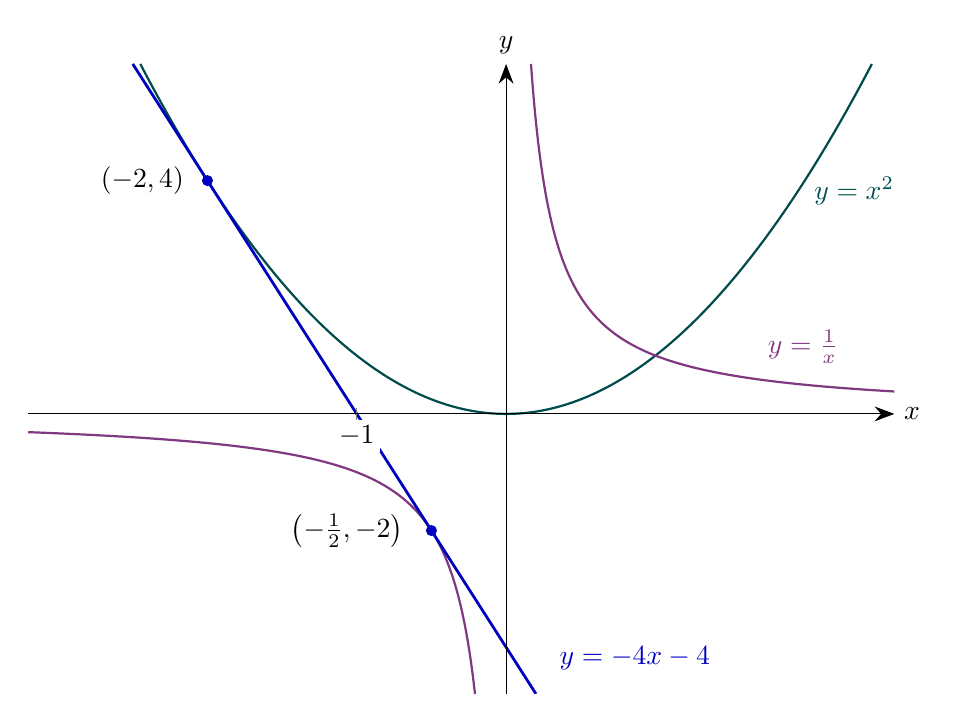
\begin{tikzpicture}
\colorlet{parabolacolour}{teal!60!black}
\colorlet{reciprocalcolour}{violet!55!gray}
\colorlet{tangentcolour}{blue!75!black}
\def\graphxmin{-3.2}
\def\graphxmax{2.6}
\def\graphymin{-4.8}
\def\graphymax{6}
\pgfmathsetmacro{\parabolaleft}{max(\graphxmin,-sqrt(\graphymax))}
\pgfmathsetmacro{\parabolaright}{min(\graphxmax,sqrt(\graphymax))}
\pgfmathsetmacro{\reciprocalnegativeend}{1/\graphymin}
\pgfmathsetmacro{\reciprocalpositivestart}{1/\graphymax}
\pgfmathsetmacro{\tangentleft}{(-\graphymax-4)/4}
\pgfmathsetmacro{\tangentright}{(-\graphymin-4)/4}
\begin{axis}[
    width=11cm,
    height=8cm,
    scale only axis,
    xmin=\graphxmin, xmax=\graphxmax,
    ymin=\graphymin, ymax=\graphymax,
    axis lines=middle,
    axis on top,
    axis line style={thin, black, -{Stealth[length=2.5mm]}},
    xtick={-1}, ytick=\empty,
    xticklabels={$-1$},
    xticklabel style={fill=white, inner sep=2pt},
    clip=true,
    clip mode=individual,
    xlabel={$x$}, ylabel={$y$},
    xlabel style={at={(axis cs:\graphxmax,0)}, anchor=west},
    ylabel style={at={(axis cs:0,\graphymax)}, anchor=south},
]
\addplot[
    thick, parabolacolour,
    domain=\parabolaleft:\parabolaright, samples=200
] {x^2};
\addplot[
    thick, reciprocalcolour,
    domain=\graphxmin:\reciprocalnegativeend, samples=250
] {1/x};
\addplot[
    thick, reciprocalcolour,
    domain=\reciprocalpositivestart:\graphxmax, samples=250
] {1/x};
\addplot[
    tangentcolour, line width=1pt,
    domain=\tangentleft:\tangentright, samples=2
] {-4*x-4};

\coordinate (ParabolaContact) at (axis cs:-2,4);
\coordinate (ReciprocalContact) at (axis cs:{-1/2},-2);
\coordinate (ParabolaLabel) at (axis cs:1.85,{1.85^2});
\coordinate (ReciprocalLabel) at (axis cs:1.65,{1/1.65});
\coordinate (TangentEnd) at (axis cs:\tangentright,\graphymin);

\fill[tangentcolour] (ParabolaContact) circle[radius=2pt];
\fill[tangentcolour] (ReciprocalContact) circle[radius=2pt];

\node[left, xshift=-5pt]
  at (ParabolaContact) {$(-2,4)$};
\node[left, xshift=-8pt, fill=white, inner sep=2pt]
  at (ReciprocalContact) {$\left(-\frac12,-2\right)$};
\node[above right, xshift=8pt, text=parabolacolour]
  at (ParabolaLabel) {$y=x^2$};
\node[above right, xshift=2pt, yshift=2pt, text=reciprocalcolour]
  at (ReciprocalLabel) {$y=\frac1x$};
\node[above right, xshift=5pt, yshift=5pt, text=tangentcolour]
  at (TangentEnd) {$y=-4x-4$};
\end{axis}
\end{tikzpicture}
% end q000774 figure F1
\end{djsSolutionFigure}

\textit{Alternative Solution:}

Let the common tangent be $y=mx+c$. Tangency means that the intersection equation for each curve has a repeated root.

The two intersection equations are
\[
\begin{aligned}
x^2=mx+c&\implies x^2-mx-c=0\\[5pt]
\frac1x=mx+c&\implies mx^2+cx-1=0
\end{aligned}
\]

Multiplying the second equation by $x$ introduces no root at $x=0$, since its constant term is $-1$. Also, $m\ne0$: the reciprocal curve has derivative $-1/x^2\ne0$, so it has no horizontal tangent.

Both equations are therefore quadratic. Setting their discriminants to zero gives
\[
m^2+4c=0
\qquad\text{and}\qquad
c^2+4m=0
\]

The first condition gives $c=-m^2/4$. Substituting into the second,
\[
\frac{m^4}{16}+4m=0
\implies m^4+64m=0
\implies m(m^3+64)=0
\]

Since $m\ne0$,
\[
m^3=-64\implies m=-4
\qquad\text{and}\qquad
c=-\frac{(-4)^2}{4}=-4
\]

Thus the common tangent is $y=-4x-4$. Setting $y=0$ gives
\[
0=-4x-4\implies x=-1
\]

Again obtaining option \textbf{C}.
% end q000774 solution
\end{djsSolution}
\end{enumerate}
\clearpage
\thispagestyle{djssolutions}
\vspace*{8pt}
\djsTopicLine{Sequences \& Series}
\begin{enumerate}[label=\textbf{\arabic*.},leftmargin=*,itemsep=0pt,start=8]
\questionitem[Sequences \& Series]
% begin q000778 stem
Five positive numbers are consecutive terms of a geometric sequence 

The middle three have sum $14$ and multiply to make $8$

What is the sum of all five numbers?
% end q000778 stem

\par\vspace*{12pt}
\begin{tabularx}{\linewidth}{@{}>{\bfseries}l Y@{}}
A &
% begin q000778 choice A
$74$
% end q000778 choice A
\\[0.8em]
B &
% begin q000778 choice B
$78$
% end q000778 choice B
\\[0.8em]
C &
% begin q000778 choice C
$80$
% end q000778 choice C
\\[0.8em]
D &
% begin q000778 choice D
$82$
% end q000778 choice D
\\[0.8em]
E &
% begin q000778 choice E
$84$
% end q000778 choice E
\\[0.8em]
F &
% begin q000778 choice F
$86$
% end q000778 choice F
\\
\end{tabularx}

\begin{djsSolution}{D}
% begin q000778 solution
Putting the middle term at the centre of the notation makes the product of the middle three easy to use. Write the five terms as
\[
\frac{b}{r^2},\quad \frac{b}{r},\quad b,\quad br,\quad br^2
\]
where $b>0$ and the common ratio $r>0$. The product of the middle three terms is
\[
\frac{b}{r}\times b\times br=8
\]

Cancelling the factors of $r$ gives
\[
b^3=8 \implies \boxed{b=2}
\]

Now use the sum of the middle three terms:
\[
\frac{2}{r}+2+2r=14 \implies r+\frac{1}{r}=6
\]


There is no need to find $r$ itself: the outer two terms require $r^2+\dfrac{1}{r^2}$ which we can obtain by squaring this result:
\[
\left(r+\frac{1}{r}\right)^2=r^2+2r\left(\frac{1}{r}\right)+\frac{1}{r^2}
\]

So
\[
36=r^2+2+\frac{1}{r^2} \implies \boxed{r^2+\frac{1}{r^2}=34}
\]


The sum of all five terms is therefore
\[
\begin{aligned}
\frac{b}{r^2}+\frac{b}{r}+b+br+br^2
&=b\left(\frac{1}{r^2}+\frac{1}{r}+1+r+r^2\right)\\[8pt]
&=2(34+6+1)=\boxed{82}
\end{aligned}
\]

The correct option is \textbf{D}.\\[5pt]

\textit{Alternative Solution:}

Avoiding the tricks used in the solution above, we can instead find the common ratio and then calculate each term. Write the five terms as

\[
a,\quad ar,\quad ar^2,\quad ar^3,\quad ar^4
\]
where $a>0$ and $r>0$.

The product of the middle three gives
\[
(ar)(ar^2)(ar^3)=a^3r^6=8
\]
so, taking cube roots,
\[
ar^2=2\quad\Longrightarrow\quad a=\frac{2}{r^2}
\]

Substituting into their sum gives
\[
\frac{2}{r}+2+2r=14
\]

Multiplying by $r$ and rearranging,
\[
r^2-6r+1=0
\]

The quadratic formula gives
\[
r=\frac{6\pm\sqrt{36-4}}{2}=3\pm2\sqrt2
\]

Take $r=3+2\sqrt2$. The first term is
\[
a=\frac{2}{(3+2\sqrt2)^2}
=\frac{2}{17+12\sqrt2}
=\frac{2(17-12\sqrt2)}{289-288}
=34-24\sqrt2
\]

Multiplying successively by $r$ gives
\[
\begin{aligned}
ar&=(34-24\sqrt2)(3+2\sqrt2)=6-4\sqrt2\\[5pt]
ar^2&=(6-4\sqrt2)(3+2\sqrt2)=2\\[5pt]
ar^3&=2(3+2\sqrt2)=6+4\sqrt2\\[5pt]
ar^4&=(6+4\sqrt2)(3+2\sqrt2)=34+24\sqrt2
\end{aligned}
\]

Since $(3+2\sqrt2)(3-2\sqrt2)=1$, the other ratio gives these same five terms in reverse order, so their sum is unchanged.

Adding, the surd terms cancel:
\[
\begin{aligned}
a+ar+ar^2+ar^3+ar^4
&=(34-24\sqrt2)+(6-4\sqrt2)+2\\[5pt]
&\quad +(6+4\sqrt2)+(34+24\sqrt2)\\[5pt]
&=34+6+2+6+34\\[5pt]
&=82
\end{aligned}
\]

The correct option is \textbf{D}.
% end q000778 solution
\end{djsSolution}
\end{enumerate}
\clearpage
\thispagestyle{djssolutions}
\vspace*{8pt}
\djsTopicLine{Probability \& Counting}
\begin{enumerate}[label=\textbf{\arabic*.},leftmargin=*,itemsep=0pt,start=9]
\questionitem[Probability \& Counting]
% begin q000767 stem
A bag contains $3$ red balls and $2$ blue balls. 

Two balls are drawn without replacement. 

If they are the same colour, both are returned to the bag. If they are different colours, both are left out.

A ball is then drawn from the bag.

What is the probability that this final ball is red?
% end q000767 stem

\par\vspace*{12pt}
\begin{tabularx}{\linewidth}{@{}>{\bfseries}l Y@{}}
A &
% begin q000767 choice A
$\dfrac{3}{5}$
% end q000767 choice A
\\[0.8em]
B &
% begin q000767 choice B
$\dfrac{19}{30}$
% end q000767 choice B
\\[0.8em]
C &
% begin q000767 choice C
$\dfrac{16}{25}$
% end q000767 choice C
\\[0.8em]
D &
% begin q000767 choice D
$\dfrac{2}{3}$
% end q000767 choice D
\\[0.8em]
E &
% begin q000767 choice E
$\dfrac{7}{10}$
% end q000767 choice E
\\
\end{tabularx}

\begin{djsSolution}{C}
% begin q000767 solution
Use a probability tree, keeping track of the balls left in the bag. Multiply along a route to find its probability, and add the probabilities of the routes we want.

First find the probabilities that the initial two balls have the same colour or different colours. There are $5$ balls for the first draw and $4$ for the second, since the first ball is not replaced.

For the same colour, the two possible routes are red then red and blue then blue:
\[
\text{Probability of same colour}
=\frac35\times\frac24+\frac25\times\frac14
=\frac25
\]

For different colours, the routes are red then blue and blue then red:
\[
\text{Probability of different colours}
=\frac35\times\frac24+\frac25\times\frac34
=\frac35
\]

These give the first branches of the tree below. To complete the tree, apply the rule in the question:
\begin{itemize}
\item Same colour: return both balls, so the bag again contains $3$ red and $2$ blue.
\item Different colours: leave both out, so the bag contains $2$ red and $1$ blue.
\end{itemize}

The final branches use these new bag contents.

\begin{djsSolutionFigure}
% begin q000767 figure F1
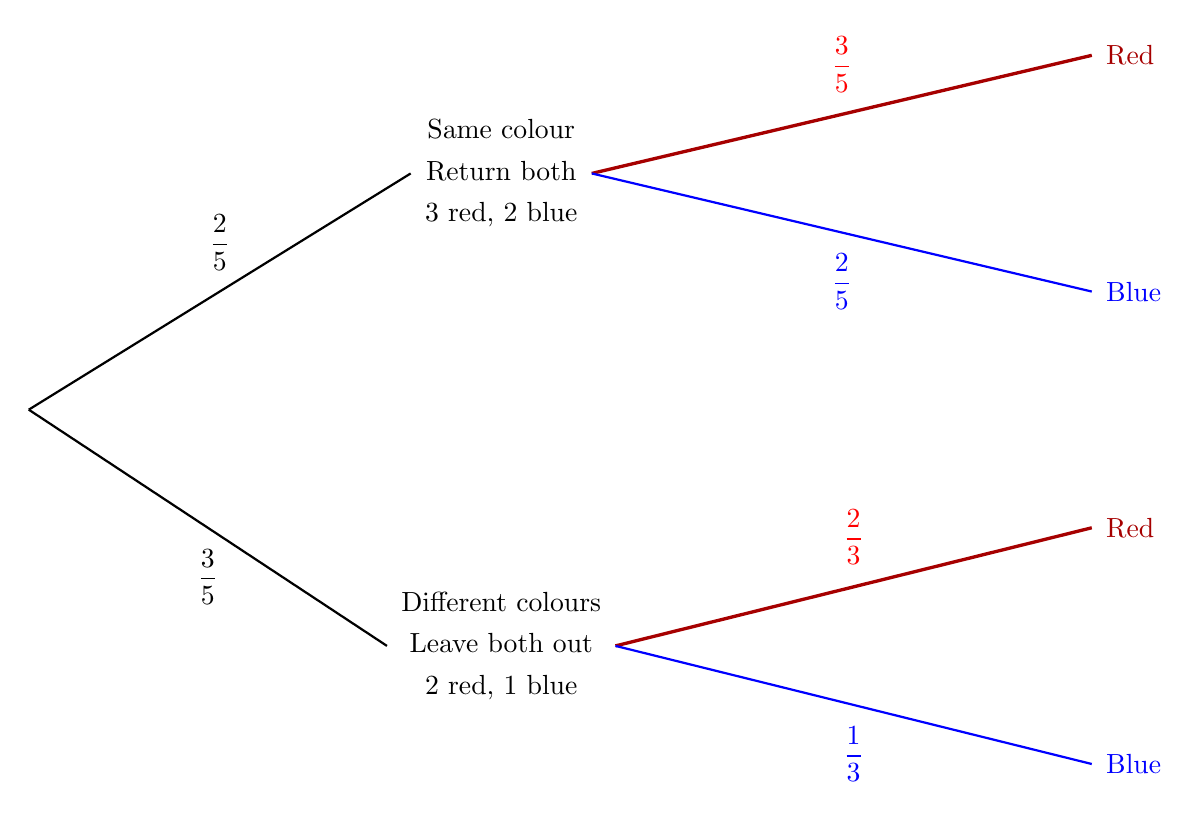
\begin{tikzpicture}[x=1.5cm,y=1.5cm,font=\normalsize]
\def\casex{4}
\def\casey{2}
\def\finalx{9}
\def\spread{1}
\pgfmathsetmacro{\outery}{\casey+\spread}
\pgfmathsetmacro{\innery}{\casey-\spread}
\coordinate (Root) at (0,0);
\coordinate (SamePosition) at (\casex,\casey);
\coordinate (DifferentPosition) at (\casex,-\casey);
\coordinate (SameRed) at (\finalx,\outery);
\coordinate (SameBlue) at (\finalx,\innery);
\coordinate (DifferentRed) at (\finalx,-\innery);
\coordinate (DifferentBlue) at (\finalx,-\outery);

\node[align=center,inner sep=5pt] (Same) at (SamePosition)
    {Same colour\\[3pt]Return both\\[3pt]3 red, 2 blue};
\node[align=center,inner sep=5pt] (Different) at (DifferentPosition)
    {Different colours\\[3pt]Leave both out\\[3pt]2 red, 1 blue};

\draw[thick,black] (Root) -- (Same.west)
    node[midway,above=4pt] {$\displaystyle\frac25$};
\draw[thick,black] (Root) -- (Different.west)
    node[midway,below=4pt] {$\displaystyle\frac35$};

\draw[line width=1.2pt,red!65!black] (Same.east) -- (SameRed)
    node[midway,above=4pt,text=red] {$\displaystyle\frac35$};
\draw[thick,blue] (Same.east) -- (SameBlue)
    node[midway,below=4pt] {$\displaystyle\frac25$};
\draw[line width=1.2pt,red!65!black] (Different.east) -- (DifferentRed)
    node[midway,above=4pt,text=red] {$\displaystyle\frac23$};
\draw[thick,blue] (Different.east) -- (DifferentBlue)
    node[midway,below=4pt] {$\displaystyle\frac13$};

\node[anchor=west,text=red!65!black,inner sep=5pt]
    at (SameRed) {Red};
\node[anchor=west,inner sep=5pt, text=blue] at (SameBlue) {Blue};
\node[anchor=west,text=red!65!black,inner sep=5pt]
    at (DifferentRed) {Red};
\node[anchor=west,inner sep=5pt, text=blue] at (DifferentBlue) {Blue};
\end{tikzpicture}
% end q000767 figure F1
\end{djsSolutionFigure}

There are two routes ending in red. Multiply along each complete route:
\[
\begin{aligned}
\text{Same colour, then final red:}\quad
&\frac25\times\frac35=\frac6{25}\\[8pt]
\text{Different colours, then final red:}\quad
&\frac35\times\frac23=\frac25
\end{aligned}
\]

Add these to obtain the probability that the final ball is red:
\[
\frac6{25}+\frac25
=\frac6{25}+\frac{10}{25}
=\boxed{\frac{16}{25}}
\]

The correct option is \textbf{C}.
% end q000767 solution
\end{djsSolution}
\end{enumerate}
\clearpage
\thispagestyle{djssolutions}
\vspace*{8pt}
\djsTopicLine{Algebra}
\begin{enumerate}[label=\textbf{\arabic*.},leftmargin=*,itemsep=0pt,start=10]
\questionitem[Algebra]
% begin q000779 stem
Real numbers $x$ and $y$ satisfy
\[x+y=xy\]
and
\[(x-1)^2+(y-1)^2=7\]

What are the possible values of $xy$?
% end q000779 stem

\par\vspace*{12pt}
\begin{tabularx}{\linewidth}{@{}>{\bfseries}l Y@{}}
A &
% begin q000779 choice A
$-5$ and $1$
% end q000779 choice A
\\[0.8em]
B &
% begin q000779 choice B
$-3$ and $3$
% end q000779 choice B
\\[0.8em]
C &
% begin q000779 choice C
$-1$ and $3$
% end q000779 choice C
\\[0.8em]
D &
% begin q000779 choice D
$-1$ and $5$
% end q000779 choice D
\\[0.8em]
E &
% begin q000779 choice E
$1$ and $5$
% end q000779 choice E
\\
\end{tabularx}

\begin{djsSolution}{D}
% begin q000779 solution
The required product is also the sum, so let $t$ denote their common value:
\[
t=x+y=xy
\]
First expand the second equation:
\[
x^2+y^2-2(x+y)+2=7
\]

To express this in terms of $t$, use the identity
\[
x^2+y^2=(x+y)^2-2xy
\]
which follows by expanding $(x+y)^2=x^2+2xy+y^2$.

Substituting the sum and product gives
\[
x^2+y^2=t^2-2t
\]

Hence the expanded second equation becomes
\[
t^2-2t-2t+2=7 \implies t^2-4t-5=0
\]

The numbers $-5$ and $1$ have product $-5$ and sum $-4$, so the factorisation is
\[
(t-5)(t+1)=0
\]

Therefore the candidate values are
\[
t=5\quad\text{or}\quad t=-1
\]
Thus 
\[
\boxed{xy=5\quad\text{or}\quad xy=-1}
\]

Option \textbf{D} is now the only possible answer, although a complete proof would also check that both values arise from real numbers $x$ and $y$ satisfying the original equations.

We can, in principle, instead explicitly solve for $x$ and $y$ and multiply to find $xy$. However this direct route involves painful algebra and, at the very least, is unsuitable for the pace demanded by the TMUA. 
% end q000779 solution
\end{djsSolution}
\end{enumerate}
\clearpage
\thispagestyle{djssolutions}
\vspace*{8pt}
\djsTopicLine{Probability \& Counting}
\begin{enumerate}[label=\textbf{\arabic*.},leftmargin=*,itemsep=0pt,start=11]
\questionitem[Probability \& Counting]
% begin q000041 stem
Find the coefficient of $x^3y^2$ in the expansion of \[(1-2x+y)^8\]
% end q000041 stem

\par\vspace*{12pt}
\begin{tabularx}{\linewidth}{@{}>{\bfseries}l Y@{}}
A &
% begin q000041 choice A
$-17920$
% end q000041 choice A
\\[0.8em]
B &
% begin q000041 choice B
$-13440$
% end q000041 choice B
\\[0.8em]
C &
% begin q000041 choice C
$-4480$
% end q000041 choice C
\\[0.8em]
D &
% begin q000041 choice D
$-560$
% end q000041 choice D
\\[0.8em]
E &
% begin q000041 choice E
$560$
% end q000041 choice E
\\[0.8em]
F &
% begin q000041 choice F
$4480$
% end q000041 choice F
\\[0.8em]
G &
% begin q000041 choice G
$17920$
% end q000041 choice G
\\
\end{tabularx}

\begin{djsSolution}{C}
% begin q000041 solution
Regard $(1-2x+y)^8$ as a product of eight identical brackets. Each bracket supplies one term, so to obtain $x^3y^2$ we must choose $-2x$ from three brackets, $y$ from two brackets, and $1$ from the remaining three.

Recall that the number of ways to choose $r$ objects from $n$ possibilities, without regard to order, is
\[
\binom{n}{r}=\frac{n!}{r!(n-r)!}
\]

Choose the three brackets supplying $-2x$, then the two supplying $y$ from the five left. The remaining brackets must supply $1$, so the number of selections is
\[
\binom83\binom52
=\frac{8\times7\times6}{3\times2\times1}
 \times\frac{5\times4}{2\times1}
=56\times10=560
\]

Each selection contributes $(-2x)^3y^2=-8x^3y^2$. Therefore the required coefficient is
\[
560\times(-8)=\boxed{-4480}
\]

The correct option is \textbf{C}.\\[5pt]

\textit{Alternative Solution 1:}

Apply the binomial theorem twice, first treating $1-2x$ as one term. Recall that
\[
(a+b)^n=\sum_{r=0}^{n}\binom{n}{r}a^{n-r}b^r
\]

With $a=1-2x$, $b=y$ and $n=8$,
\[
\bigl((1-2x)+y\bigr)^8
=\sum_{r=0}^{8}\binom{8}{r}(1-2x)^{8-r}y^r
\]

Only $r=2$ can give $y^2$, since the remaining power contains no $y$. The relevant term is therefore
\[
\binom82(1-2x)^6y^2
\]

Now apply the binomial theorem to the remaining power:
\[
(1-2x)^6
=\sum_{r=0}^{6}\binom6r1^{6-r}(-2x)^r
\]

Only $r=3$ gives $x^3$, with coefficient $\binom63(-2)^3$. Hence the coefficient of $x^3y^2$ in the original expansion is
\[
\binom82\binom63(-2)^3
=28\times20\times(-8)
=-4480
\]

Again obtaining option \textbf{C}.\\[5pt]

\textit{Alternative Solution 2:}

The trinomial theorem gives a short calculation here, but is not needed for either of the preceding methods. Note that the trinomial theorem is far beyond the TMUA specification.

For a non-negative integer $n$, it states that
\[
(a+b+c)^n
=\sum_{i+j+k=n}\frac{n!}{i!j!k!}a^ib^jc^k
\]

The sum runs over all non-negative integers $i$, $j$ and $k$ whose total is $n$. These are the respective exponents of $a$, $b$ and $c$. A zero exponent is allowed, with $0!=1$.

Substituting $a=1$, $b=-2x$, $c=y$ and $n=8$ gives
\[
(1-2x+y)^8
=\sum_{i+j+k=8}\frac{8!}{i!j!k!}1^i(-2x)^jy^k
\]

To obtain $x^3y^2$, we need $j=3$ and $k=2$, so $i=8-3-2=3$. The required coefficient is therefore
\[
\frac{8!}{3!3!2!}(-2)^3
=\frac{8\times7\times6\times5\times4}{(3\times2\times1)(2\times1)}(-8)
=560(-8)
=-4480
\]

The correct option is \textbf{C}.\\[5pt]

\textit{Remark:} (Optional)

The trinomial theorem extends the binomial theorem from two terms to three. More generally, the \emph{multinomial theorem} applies to a sum of $m$ terms:
\[
(a_1+\cdots+a_m)^n
=\sum_{i_1+\cdots+i_m=n}
\frac{n!}{i_1!\cdots i_m!}
a_1^{i_1}\cdots a_m^{i_m}
\]

Here $m$ is the number of terms in the bracket, and $n$ is a non-negative integer. The sum runs over all non-negative integer exponents $i_1,\ldots,i_m$ whose total is $n$.

Each exponent records how many of the $n$ brackets supply the corresponding term. The factorial expression counts the ways to make those selections.

Taking $m=3$, with $a_1=a$, $a_2=b$ and $a_3=c$, gives the trinomial theorem. Taking $m=2$ gives
\[
(a+b)^n=\sum_{i+j=n}\frac{n!}{i!j!}a^ib^j
\]

Since $i+j=n$, choosing $j$ fixes $i=n-j$. We can therefore write the sum using $j$ alone:
\[
(a+b)^n
=\sum_{j=0}^{n}\frac{n!}{(n-j)!j!}a^{n-j}b^j
=\sum_{j=0}^{n}\binom nj a^{n-j}b^j
\]

The summation index is a dummy variable: its name does not change the sum. Renaming $j$ as $r$ gives exactly the binomial theorem quoted above:
\[
(a+b)^n=\sum_{r=0}^{n}\binom nr a^{n-r}b^r
\]

Thus the multinomial theorem includes both the binomial and trinomial theorems.
% end q000041 solution
\end{djsSolution}
\end{enumerate}
\clearpage
\thispagestyle{djssolutions}
\vspace*{8pt}
\djsTopicLine{Inequalities}
\begin{enumerate}[label=\textbf{\arabic*.},leftmargin=*,itemsep=0pt,start=12]
\questionitem[Inequalities]
% begin q000773 stem
The function $f$ is defined for all real $x$ by
\[
f(x)=\frac{x^{2}+4x+1}{x^{2}+1}
\]

Which of the following gives all possible values of \(f(x)\) as \(x\) varies over the real numbers?
% end q000773 stem

\par\vspace*{12pt}
\begin{tabularx}{\linewidth}{@{}>{\bfseries}l Y@{}}
A &
% begin q000773 choice A
$-1 \le f(x) \le 3$
% end q000773 choice A
\\[0.8em]
B &
% begin q000773 choice B
$f(x) \le -1$ or $f(x) \ge 3$
% end q000773 choice B
\\[0.8em]
C &
% begin q000773 choice C
$1 \le f(x) \le 3$
% end q000773 choice C
\\[0.8em]
D &
% begin q000773 choice D
$-3 \le f(x) \le 1$
% end q000773 choice D
\\[0.8em]
E &
% begin q000773 choice E
$-1 \le f(x) \le 1$
% end q000773 choice E
\\[0.8em]
F &
% begin q000773 choice F
$f(x)$ can take all real values
% end q000773 choice F
\\
\end{tabularx}

\begin{djsSolution}{A}
% begin q000773 solution
Put $y=f(x)$ and find which values of $y$ allow a real input $x$. Since $x^2+1>0$ for every real $x$, multiplying by the denominator gives
\[
y(x^2+1)=x^2+4x+1
\]

Rearranging as an equation in $x$,
\[
(y-1)x^2-4x+(y-1)=0
\]

First suppose $y\ne1$, so this is a quadratic. A quadratic $ax^2+bx+c=0$, with $a\ne0$, has at least one real root exactly when its discriminant satisfies
\[
b^2-4ac\ge0
\]

Here the discriminant is
\[
\begin{aligned}
b^2-4ac
&=(-4)^2-4(y-1)(y-1)\\[5pt]
&=16-4(y-1)^2
\end{aligned}
\]

Therefore a real input exists exactly when
\[
16-4(y-1)^2\ge0
\]

Rearranging,
\[
(y-1)^2\le4
\]

Taking the bounds on $y-1$,
\[
-2\le y-1\le2
\]

Adding $1$,
\[
-1\le y\le3
\]

The endpoints are included because a zero discriminant gives a repeated real root. At either endpoint, that root is
\[
x=\frac{-(-4)}{2(y-1)}
\]

Substituting the endpoint values,
\[
\begin{aligned}
y=-1 &: \quad x=\frac{4}{2(-2)}=-1\\[8pt]
y=3 &: \quad x=\frac{4}{2(2)}=1
\end{aligned}
\]

Now check $y=1$ separately, since the quadratic coefficient then vanishes. Substituting into the rearranged equation gives
\[
-4x=0
\]

Hence
\[
x=0
\]

So $y=1$ is also attained. Every value between $-1$ and $3$ gives a real solution of the rearranged equation, and multiplying by the positive denominator was reversible, so every such solution is an input with $f(x)=y$.

No value outside these bounds gives a real input. Thus all possible values are
\[
-1\le f(x)\le3
\]

The correct option is \textbf{A}.\\[5pt]

\textit{Alternative Solution:}

This approach uses rational-function analysis and the quotient rule, which are beyond the TMUA specification but might be familiar to some candidates. 

The question asks for the \emph{range} of $f$: all output values it can take, or equivalently all heights reached by its graph.

There are no vertical asymptotes because $x^2+1>0$. The numerator and denominator have the same degree and leading coefficient, so the horizontal asymptote at both ends is $y=1$.

Also,
\[
f(x)=1+\frac{4x}{x^2+1}
\]
shows that the graph lies below $y=1$ for $x<0$, above it for $x>0$, and crosses it at $(0,1)$.

For a quotient $y= u(x)/v(x)$, the quotient rule states that
\[
\frac{\mathrm{d}y}{\mathrm{d}x}
=\frac{u'(x)v(x)-u(x)v'(x)}{[v(x)]^2}
\]

Applying it here,
\[
\begin{aligned}
f'(x)
&=\frac{(x^2+1)(2x+4)-(x^2+4x+1)(2x)}{(x^2+1)^2}\\[8pt]
&=\frac{4(1-x^2)}{(x^2+1)^2}
\end{aligned}
\]

Hence
\[
f'(x)=0\implies x=\pm1
\qquad\text{with}\qquad
f(-1)=-1,\quad f(1)=3
\]

The derivative is negative for $x<-1$, positive for $-1<x<1$, and negative for $x>1$. Together with the horizontal asymptote, this gives the following sketch.

\begin{djsSolutionFigure}
% begin q000773 figure F2
\begin{tikzpicture}[x=0.7cm,y=1.65cm]
\def\xmin{-11.5}
\def\xmax{11.5}
\def\ymin{-1.6}
\def\ymax{3.7}
\def\plotmin{-11.5}
\def\plotmax{11.5}
\def\minx{-1}
\def\maxx{1}
\pgfmathsetmacro{\miny}{((\minx)^2+4*(\minx)+1)/((\minx)^2+1)}
\pgfmathsetmacro{\maxy}{((\maxx)^2+4*(\maxx)+1)/((\maxx)^2+1)}
\coordinate (Minimum) at (\minx,\miny);
\coordinate (Maximum) at (\maxx,\maxy);
\coordinate (XEnd) at (\xmax,0);
\coordinate (YEnd) at (0,\ymax);
\coordinate (AsymptoteLabel) at (\plotmax,1);
\def\labelx{4.5}
\pgfmathsetmacro{\labely}{((\labelx)^2+4*(\labelx)+1)/((\labelx)^2+1)}
\coordinate (CurveLabel) at (\labelx,\labely);

\draw[thin,dashed,black] (\xmin,1) -- (\xmax,1);
\draw[thick,black] (\xmin,0) -- (XEnd);
\draw[thick,black] (0,\ymin) -- (YEnd);
\node[right=3pt] at (XEnd) {$x$};
\node[above=3pt] at (YEnd) {$y$};

\draw[teal,line width=1.5pt]
  plot[domain=\plotmin:\plotmax,samples=401,variable=\t]
    (\t,{((\t)^2+4*(\t)+1)/((\t)^2+1)});

\fill[teal] (Minimum) circle[radius=2.6pt];
\fill[teal] (Maximum) circle[radius=2.6pt];
\node[below left=5pt] at (Minimum) {$(-1,-1)$};
\node[above right=5pt] at (Maximum) {$(1,3)$};
\node[below left=4pt] at (AsymptoteLabel) {$y=1$};
\node[above right=5pt] at (CurveLabel) {$y=f(x)$};
\end{tikzpicture}
% end q000773 figure F2
\end{djsSolutionFigure}

The minimum is $-1$, the maximum is $3$, and continuity ensures that every value between them occurs. Therefore the range is
\[
-1\le f(x)\le3
\]

The correct option is \textbf{A}.
% end q000773 solution
\end{djsSolution}
\end{enumerate}
\clearpage
\thispagestyle{djssolutions}
\vspace*{8pt}
\djsTopicLine{Coordinate Geometry}
\begin{enumerate}[label=\textbf{\arabic*.},leftmargin=*,itemsep=0pt,start=13]
\questionitem[Coordinate Geometry]
% begin q000620 stem
The points $P$ and $R$ lie on the curve $y=x^2$ and have $x$-coordinates $1$ and $3$, respectively. The tangents to the curve at $P$ and $R$ meet at $Q$.

The area enclosed by the curve and the line segment $PR$ is $A$. The area of triangle $PQR$ is $B$.

What is the value of $\dfrac{A}{B}$?
% end q000620 stem

\begin{center}
% begin q000620 diagram
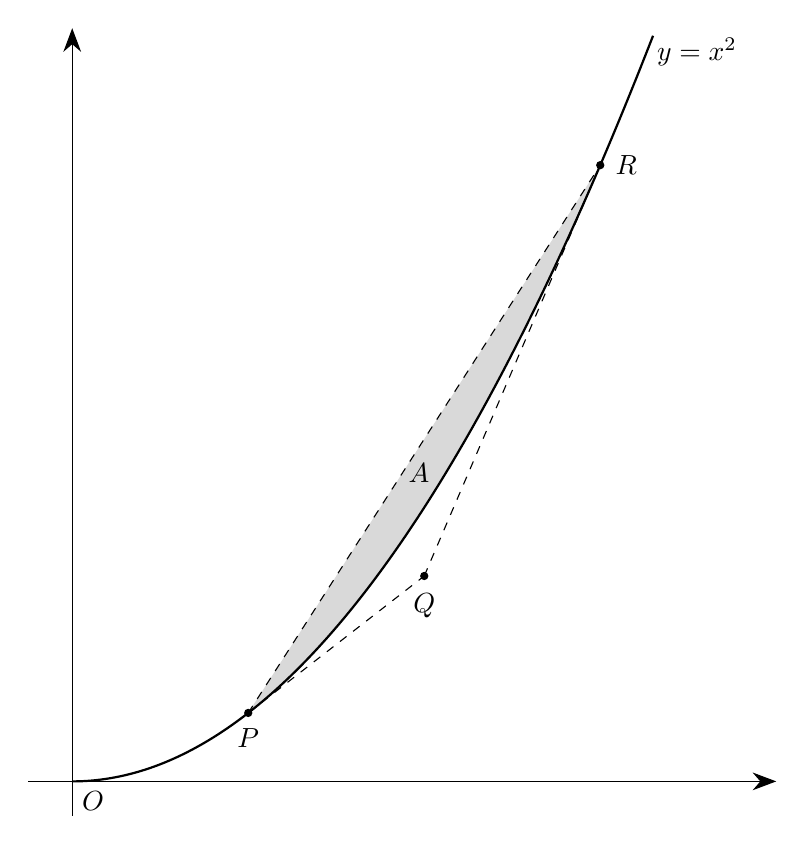
\begin{tikzpicture}
\begin{axis}[
    width=9.5cm,
    height=10cm,
    scale only axis,
    axis lines=middle,
    axis line style={solid, black, -{Stealth[length=3mm]}},
    axis on top,
    xmin=-0.25, xmax=4,
    ymin=-0.5, ymax=11,
    xtick=\empty,
    ytick=\empty,
    clip=true,
    clip mode=individual
]
% Exact paths defining the shaded region
\addplot[draw=none, name path=chord, domain=1:3, samples=2] {4*x-3};
\addplot[draw=none, name path=parabolaRegion, domain=1:3, samples=100] {x^2};
\addplot[gray!30] fill between[of=chord and parabolaRegion];

% Parabola and triangle boundary
\addplot[thick, black, domain=0:3.3, samples=150] {x^2}
    node[pos=0.98, right] {$y=x^2$};
\addplot[dashed, black, domain=1:3, samples=2] {4*x-3};
\addplot[dashed, black, domain=1:2, samples=2] {2*x-1};
\addplot[dashed, black, domain=2:3, samples=2] {6*x-9};

% Marked points
\fill (axis cs:1,1) circle (1.5pt);
\fill (axis cs:2,3) circle (1.5pt);
\fill (axis cs:3,9) circle (1.5pt);
\node[right=2pt, below=2pt] at (axis cs:1,1) {$P$};
\node[below=3pt] at (axis cs:2,3) {$Q$};
\node[right=2pt] at (axis cs:3,9) {$R$};

% Region and origin labels
\node at (axis cs:1.97,4.5) {$A$};
\node[below right] at (axis cs:0,0) {$O$};
\end{axis}
\end{tikzpicture}
% end q000620 diagram
\end{center}

\par\vspace*{12pt}
\begin{tabularx}{\linewidth}{@{}>{\bfseries}l Y@{}}
A &
% begin q000620 choice A
$\dfrac{1}{3}$
% end q000620 choice A
\\[0.8em]
B &
% begin q000620 choice B
$\dfrac{1}{2}$
% end q000620 choice B
\\[0.8em]
C &
% begin q000620 choice C
$\dfrac{2}{3}$
% end q000620 choice C
\\[0.8em]
D &
% begin q000620 choice D
$\dfrac{3}{4}$
% end q000620 choice D
\\[0.8em]
E &
% begin q000620 choice E
$\dfrac{3}{2}$
% end q000620 choice E
\\
\end{tabularx}

\begin{djsSolution}{C}
% begin q000620 solution
Substituting into $y=x^2$ gives
\[
P=(1,1),\qquad R=(3,9)
\]

The gradient of $PR$ is $(9-1)/(3-1)=4$, so its equation is
\[
y-1=4(x-1)\implies y=4x-3
\]

Since $\mathrm{d}y/\mathrm{d}x=2x$, the tangent gradients at $P$ and $R$ are $2$ and $6$. Hence
\[
\begin{aligned}
\text{At }P:\quad y-1&=2(x-1)\implies y=2x-1\\[5pt]
\text{At }R:\quad y-9&=6(x-3)\implies y=6x-9
\end{aligned}
\]

At their intersection,
\[
2x-1=6x-9\implies x=2,\qquad y=3
\]
so $Q=(2,3)$.

First calculate $A$. The chord lies above the curve between $P$ and $R$, so integrate upper minus lower:
\[
\begin{aligned}
A&=\int_1^3\bigl((4x-3)-x^2\bigr)\,\mathrm{d}x\\[8pt]
&=\left[2x^2-3x-\frac{x^3}{3}\right]_1^3\\[8pt]
&=0-\left(-\frac43\right)=\frac43
\end{aligned}
\]

For $B$, draw the vertical segment from $Q$ to the chord, meeting it at $S$. Substituting $x=2$ into $y=4x-3$ gives $S=(2,5)$, so $QS=2$.

The diagram below isolates triangle $PQR$. The two shaded triangles share the vertical base $QS$. Their perpendicular heights are the horizontal distances from $P$ and $R$ to the line $x=2$, both equal to $1$.

\begin{djsSolutionFigure}
% begin q000620 figure F1
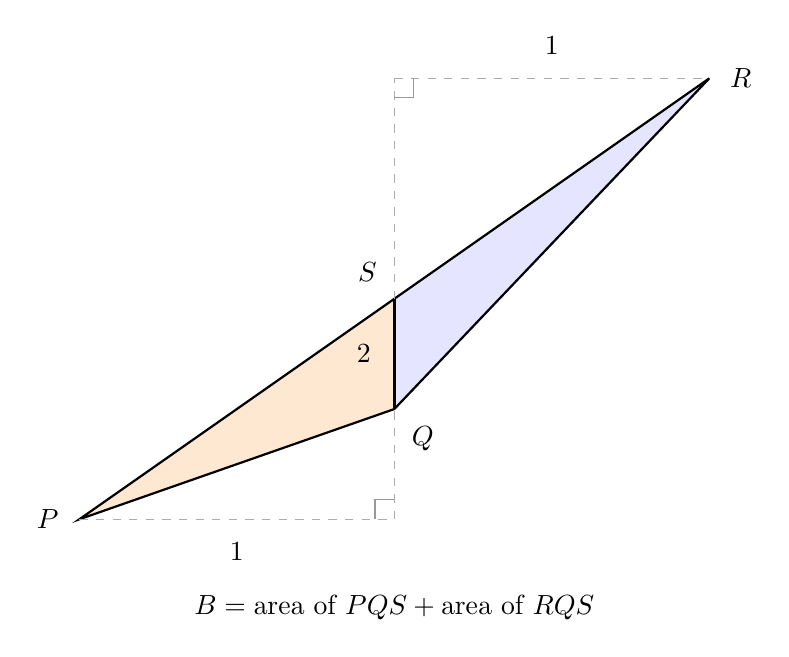
\begin{tikzpicture}[x=4cm,y=0.7cm]
\coordinate (P) at (1,1);
\coordinate (Q) at (2,3);
\coordinate (R) at (3,9);
\coordinate (S) at (2,5);
\coordinate (H) at (2,1);
\coordinate (K) at (2,9);

% Exact paths defining the two parts of triangle B
\fill[orange!18] (P) -- (Q) -- (S) -- cycle;
\fill[blue!10] (R) -- (Q) -- (S) -- cycle;

% Highlighted boundary of triangle B
\draw[thick,black] (P) -- (Q) -- (R) -- cycle;

% Exact vertices and the vertical subdivision
\draw[gray!65,dashed] (H) -- (Q);
\draw[gray!65,dashed] (S) -- (K);
\draw[very thick,black] (Q) -- (S);
\draw[gray!65,dashed] (P) -- (H)
  node[midway,below=5pt,text=black] {$1$};
\draw[gray!65,dashed] (K) -- (R)
  node[midway,above=5pt,text=black] {$1$};

\draw[thin,gray!80]
  ([xshift=-7pt]H) -- ([xshift=-7pt,yshift=7pt]H)
  -- ([yshift=7pt]H);
\draw[thin,gray!80]
  ([xshift=7pt]K) -- ([xshift=7pt,yshift=-7pt]K)
  -- ([yshift=-7pt]K);

% Vertex labels
\node[left=4pt] at (P) {$P$};
\node[below right=4pt] at (Q) {$Q$};
\node[right=4pt] at (R) {$R$};
\node[above left=4pt] at (S) {$S$};

% Common base and total area labels
\path (Q) -- (S) node[midway,left=5pt] {$2$};
\node[below=24pt] at (H)
  {$B=\text{area of }PQS+\text{area of }RQS$};
\end{tikzpicture}
% end q000620 figure F1
\end{djsSolutionFigure}

Using $\text{area}=\frac12\times\text{base}\times\text{perpendicular height}$ for each triangle,
\[
B=\frac12\times2\times1+\frac12\times2\times1=2
\]

Therefore
\[
\frac{A}{B}=\frac{\frac43}{2}=\frac23
\]

The correct option is \textbf{C}.\\[5pt]

\textit{Alternative Solution:} (Other formulae for $B$)

The following triangle-area formulae are beyond the specification. We reuse $P=(1,1)$, $Q=(2,3)$, $R=(3,9)$ and $A=\frac43$ from the primary solution.

For two side vectors $\begin{pmatrix}u_1\\u_2\end{pmatrix}$ and $\begin{pmatrix}v_1\\v_2\end{pmatrix}$ starting at the same vertex, the triangle's area is
\[
\text{area}=\frac12\Bigl|u_1v_2-u_2v_1\Bigr|
\]

This is half the magnitude of their cross product. Here $\overrightarrow{PQ}=\begin{pmatrix}1\\2\end{pmatrix}$ and $\overrightarrow{PR}=\begin{pmatrix}2\\8\end{pmatrix}$, so
\[
B=\frac12\Bigl|1\times8-2\times2\Bigr|=2
\]

Alternatively, for vertices $(x_1,y_1)$, $(x_2,y_2)$ and $(x_3,y_3)$, the \emph{shoelace formula} is
\[
\text{area}
=\frac12\Bigl|
(x_1y_2+x_2y_3+x_3y_1)
-(y_1x_2+y_2x_3+y_3x_1)
\Bigr|
\]

Using the vertices in the order $P$, $Q$, $R$,
\[
B=\frac12\Bigl|(1\times3+2\times9+3\times1)
-(1\times2+3\times3+9\times1)\Bigr|
=\frac12\bigl|24-20\bigr|=2
\]

Either calculation gives
\[
\frac{A}{B}=\frac{\frac43}{2}=\frac23
\]

The correct option is \textbf{C}. \\[5pt]

\textit{Remark:} (Optional, the shoelace formula)

The shoelace formula works for any polygon whose sides do not cross. List its vertices $(x_1,y_1),\ldots,(x_n,y_n)$ in order around the boundary, clockwise or anticlockwise, and repeat the first vertex at the end. Then
\[
\text{area}
=\frac12\Bigl|
\sum_{i=1}^{n}x_i y_{i+1}
-\sum_{i=1}^{n}y_i x_{i+1}
\Bigr|
\qquad
(x_{n+1},y_{n+1})=(x_1,y_1)
\]

For example, consider this pentagon.

\begin{djsSolutionFigure}
% begin q000620 figure F2
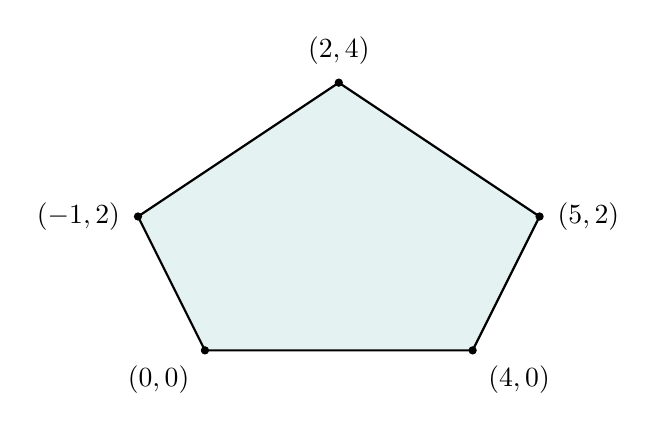
\begin{tikzpicture}[x=0.85cm,y=0.85cm]
\coordinate (A) at (0,0);
\coordinate (B) at (4,0);
\coordinate (C) at (5,2);
\coordinate (D) at (2,4);
\coordinate (E) at (-1,2);

\fill[teal!10] (A) -- (B) -- (C) -- (D) -- (E) -- cycle;
\draw[thick,black] (A) -- (B) -- (C) -- (D) -- (E) -- cycle;

\foreach \point in {A,B,C,D,E} {
  \fill[black] (\point) circle[radius=1.5pt];
}

\node[below left=3pt] at (A) {$(0,0)$};
\node[below right=3pt] at (B) {$(4,0)$};
\node[right=3pt] at (C) {$(5,2)$};
\node[above=3pt] at (D) {$(2,4)$};
\node[left=3pt] at (E) {$(-1,2)$};
\end{tikzpicture}
% end q000620 figure F2
\end{djsSolutionFigure}

Write the coordinates in boundary order, repeating the first pair:
\[
\begin{array}{c|r}
x&y\\ \hline
0&0\\
4&0\\
5&2\\
2&4\\
-1&2\\
0&0
\end{array}
\]

Multiply each left-hand entry by the next right-hand entry and add; then do the same in the opposite direction. 

\begin{djsSolutionFigure}
% begin q000620 figure F3
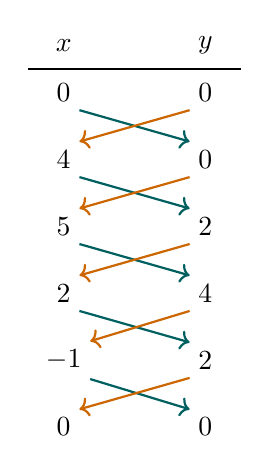
\begin{tikzpicture}[x=1.8cm,y=0.85cm]
\node at (0,0.7) {$x$};
\node at (1,0.7) {$y$};
\draw[thin] (-0.25,0.35) -- (1.25,0.35);

\foreach \row/\xvalue/\yvalue in {0/0/0,1/4/0,2/5/2,3/2/4,4/-1/2,5/0/0} {
  \node[inner sep=3pt] (X\row) at (0,-\row) {$\xvalue$};
  \node[inner sep=3pt] (Y\row) at (1,-\row) {$\yvalue$};
}

\foreach \row in {0,1,2,3,4} {
  \pgfmathtruncatemacro{\nextrow}{\row+1}
  \draw[->,thick,teal!75!black]
    (X\row.south east) -- (Y\nextrow.north west);
  \draw[->,thick,orange!80!black]
    (Y\row.south west) -- (X\nextrow.north east);
}
\end{tikzpicture}
% end q000620 figure F3
\end{djsSolutionFigure}
These crossing products give the formula its name:
\[
\begin{aligned}
\text{area}
&=\frac12\Bigl|
\textcolor{teal!75!black}{\bigl(0(0)+4(2)+5(4)+2(2)+(-1)(0)\bigr)}\\
&\qquad\quad
-\textcolor{orange!80!black}{\bigl(0(4)+0(5)+2(2)+4(-1)+2(0)\bigr)}
\Bigr|\\[5pt]
&=\frac12\bigl|32-0\bigr|
=16
\end{aligned}
\]

So the area of the pentagon is $16$.
% end q000620 solution
\end{djsSolution}
\end{enumerate}
\clearpage
\thispagestyle{djssolutions}
\vspace*{8pt}
\djsTopicLine{Integration}
\begin{enumerate}[label=\textbf{\arabic*.},leftmargin=*,itemsep=0pt,start=14]
\questionitem[Integration]
% begin q000627 stem
The diagram shows the graph of $y=f(x)$ for $0\le x\le 8$. The graph is made up of straight line segments joining the points $(0,2)$, $(2,2)$, $(5,-4)$, $(6,0)$ and $(8,1)$.

The function $g$ is defined by
\[g(x)=\int_0^x f(t)\,\mathrm{d}t \qquad \text{for } 0\le x\le 8\]

How many values of $x$ with $0\le x\le 8$ satisfy $g(x)=0$?
% end q000627 stem

\begin{center}
% begin q000627 diagram
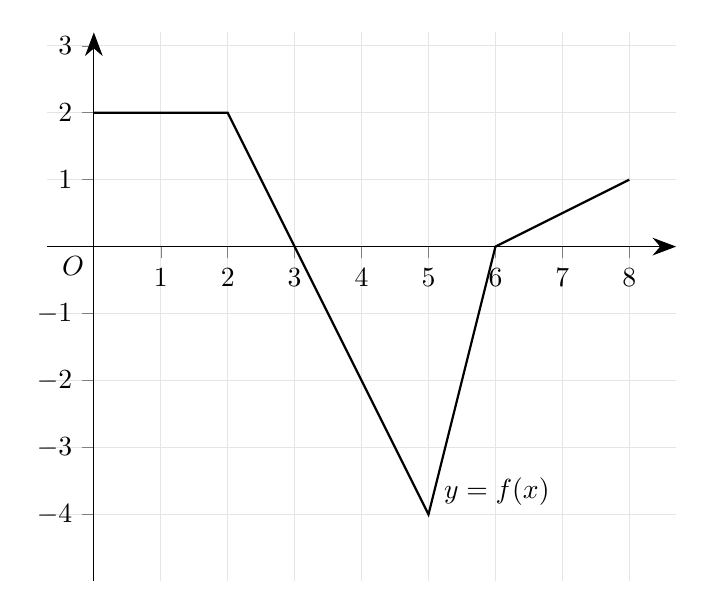
\begin{tikzpicture}
\begin{axis}[
    x=0.85cm,
    y=0.85cm,
    scale only axis,
    axis lines=middle,
    axis line style={-{Stealth[length=3mm]}, black},
    xmin=-0.7, xmax=8.7,
    ymin=-5, ymax=3.2,
    xtick={0,1,2,3,4,5,6,7,8},
    xticklabels={,$1$,$2$,$3$,$4$,$5$,$6$,$7$,$8$},
    ytick={-4,-3,-2,-1,0,1,2,3},
    yticklabels={$-4$,$-3$,$-2$,$-1$,,$1$,$2$,$3$},
    tick align=outside,
    grid=major,
    grid style={gray!20, thin},
    clip=true
]

\addplot[
    thick,
    black,
    mark=none
] coordinates {
    (0,2) (2,2) (5,-4) (6,0) (8,1)
} node[pos=0.6, below right, yshift=9pt] {$y=f(x)$};

\node[below left] at (axis cs:0,0) {$O$};
\node[right] at (axis cs:8.7,0) {$x$};
\node[above] at (axis cs:0,3.2) {$y$};

\end{axis}
\end{tikzpicture}
% end q000627 diagram
\end{center}

\par\vspace*{12pt}
\begin{tabularx}{\linewidth}{@{}>{\bfseries}l Y@{}}
A &
% begin q000627 choice A
$0$
% end q000627 choice A
\\[0.8em]
B &
% begin q000627 choice B
$1$
% end q000627 choice B
\\[0.8em]
C &
% begin q000627 choice C
$2$
% end q000627 choice C
\\[0.8em]
D &
% begin q000627 choice D
$3$
% end q000627 choice D
\\[0.8em]
E &
% begin q000627 choice E
$4$
% end q000627 choice E
\\[0.8em]
F &
% begin q000627 choice F
$5$
% end q000627 choice F
\\
\end{tabularx}

\begin{djsSolution}{D}
% begin q000627 solution
$g(x)$ is the accumulated signed area from $0$ to $x$: area above the axis is added, and area below it is subtracted. We want the points where these areas balance.

First, $g(0)=0$, so $x=0$ is one solution.

The area of a trapezium is
\[
\text{area}=\frac12(a+b)h
\]
where $a$ and $b$ are the lengths of the parallel sides and $h$ is the perpendicular distance between them.

From $0$ to $3$, the positive region is a trapezium with parallel sides of lengths $2$ and $3$, separated by a distance of $2$. Hence
\[
g(3)=\frac12(2+3)\times2=5
\]

Only positive area is added over this interval, so there is no further zero before $x=3$.

The diagram summarises the three signed areas.

\begin{djsSolutionFigure}
% begin q000627 figure F1
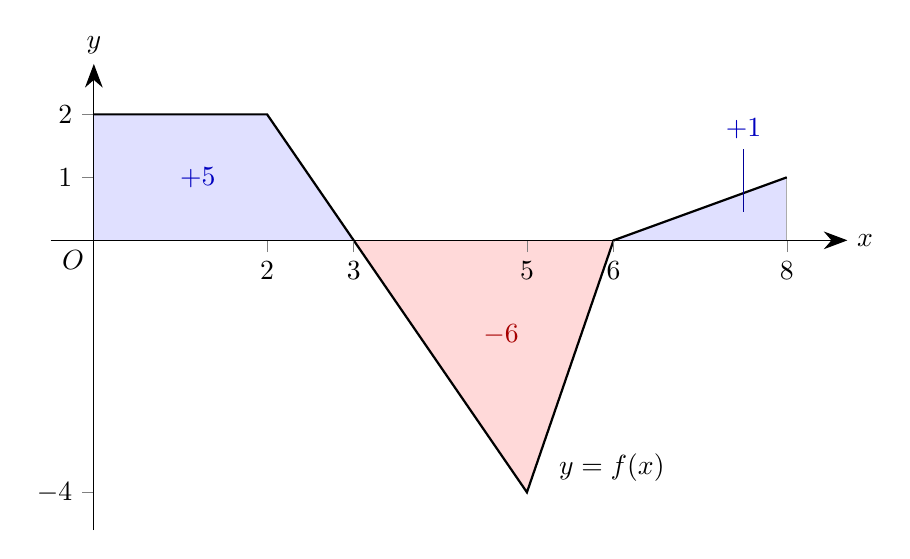
\begin{tikzpicture}
\begin{axis}[
    x=1.1cm,
    y=0.8cm,
    scale only axis,
    axis lines=middle,
    axis line style={-{Stealth[length=3mm]}, black},
    axis on top,
    xmin=-0.5, xmax=8.7,
    ymin=-4.6, ymax=2.8,
    xtick={2,3,5,6,8},
    ytick={-4,1,2},
    tick align=outside,
    clip=true,
    clip mode=individual
]

\path[fill=blue!12,draw=none]
    (axis cs:0,0) -- (axis cs:0,2)
    -- (axis cs:2,2) -- (axis cs:3,0) -- cycle;
\path[fill=red!15,draw=none]
    (axis cs:3,0) -- (axis cs:5,-4)
    -- (axis cs:6,0) -- cycle;
\path[fill=blue!12,draw=none]
    (axis cs:6,0) -- (axis cs:8,1)
    -- (axis cs:8,0) -- cycle;

\draw[thin,gray!65] (axis cs:8,0) -- (axis cs:8,1);

\addplot[thick,black,mark=none] coordinates {
    (0,2) (2,2) (5,-4) (6,0) (8,1)
};

\node[text=blue!75!black] at (axis cs:1.2,1) {$+5$};
\node[text=red!65!black] at (axis cs:4.7,-1.5) {$-6$};

\draw[thin,blue!60!black]
    (axis cs:7.5,1.45) -- (axis cs:7.5,0.45);
\node[above,text=blue!75!black] at (axis cs:7.5,1.45) {$+1$};

\node[right=5pt] at (axis cs:5.1,-3.6) {$y=f(x)$};
\node[below left] at (axis cs:0,0) {$O$};
\node[right] at (axis cs:8.7,0) {$x$};
\node[above] at (axis cs:0,2.8) {$y$};

\end{axis}
\end{tikzpicture}
% end q000627 figure F1
\end{djsSolutionFigure}

From $3$ to $5$, the area subtracted is $\frac12\times2\times4=4$, leaving
\[
g(5)=5-4=1
\]

From $5$ to $6$, the total area available to subtract is $\frac12\times1\times4=2$. Only an area of $1$ is needed to cancel the remaining positive balance.

As we move right from $5$ to $6$, the area subtracted grows from $0$ to $2$, so it reaches $1$ exactly once. Call that position $c$, as shown in the sketch:

\begin{djsSolutionFigure}
% begin q000627 figure F2
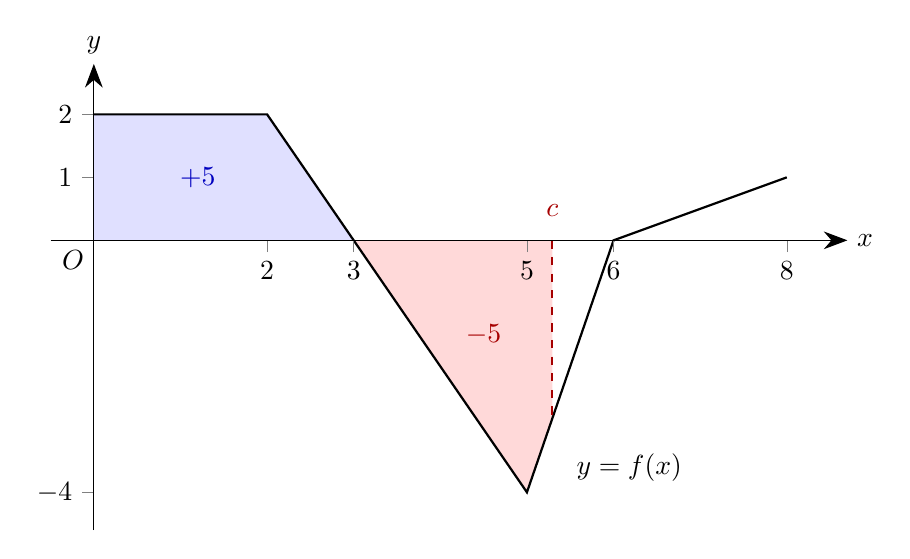
\begin{tikzpicture}
\pgfmathsetmacro{\balancex}{6-1/sqrt(2)}
\pgfmathsetmacro{\balancey}{4*\balancex-24}
\begin{axis}[
    x=1.1cm,
    y=0.8cm,
    scale only axis,
    axis lines=middle,
    axis line style={-{Stealth[length=3mm]}, black},
    axis on top,
    xmin=-0.5, xmax=8.7,
    ymin=-4.6, ymax=2.8,
    xtick={2,3,5,6,8},
    ytick={-4,1,2},
    tick align=outside,
    clip=true,
    clip mode=individual
]

\path[fill=blue!12,draw=none]
    (axis cs:0,0) -- (axis cs:0,2)
    -- (axis cs:2,2) -- (axis cs:3,0) -- cycle;
\path[fill=red!15,draw=none]
    (axis cs:3,0) -- (axis cs:5,-4)
    -- (axis cs:\balancex,\balancey)
    -- (axis cs:\balancex,0) -- cycle;

\addplot[thick,black,mark=none] coordinates {
    (0,2) (2,2) (5,-4) (6,0) (8,1)
};

\draw[thick,dashed,red!65!black]
    (axis cs:\balancex,0) -- (axis cs:\balancex,\balancey);
\node[above=5pt,text=red!65!black]
    at (axis cs:\balancex,0) {$c$};

\node[text=blue!75!black] at (axis cs:1.2,1) {$+5$};
\node[text=red!65!black] at (axis cs:4.5,-1.5) {$-5$};

\node[right=5pt] at (axis cs:5.3,-3.6) {$y=f(x)$};
\node[below left] at (axis cs:0,0) {$O$};
\node[right] at (axis cs:8.7,0) {$x$};
\node[above] at (axis cs:0,2.8) {$y$};

\end{axis}
\end{tikzpicture}
% end q000627 figure F2
\end{djsSolutionFigure}

After $c$, more negative area is added, giving
\[
g(6)=1-2=-1
\]

Finally, the positive triangle from $6$ to $8$ has area
$
\frac12\times2\times1=1
$. All of this area is needed to cancel the deficit, so the balance returns to zero only at $x=8$.

There are therefore $3$ solutions: $x=0$, one value between $5$ and $6$, and $x=8$. The correct option is \textbf{D}.
% end q000627 solution
\end{djsSolution}
\end{enumerate}
\clearpage
\thispagestyle{djssolutions}
\vspace*{8pt}
\djsTopicLine{Number}
\begin{enumerate}[label=\textbf{\arabic*.},leftmargin=*,itemsep=0pt,start=15]
\questionitem[Number]
% begin q000725 stem
Let $k$ be a positive integer, and let $N=2^4\times3^k$

The product of all the positive factors of $N$ is the fourth power of an integer. 

What is the smallest possible value of $k$?
% end q000725 stem

\par\vspace*{12pt}
\begin{tabularx}{\linewidth}{@{}>{\bfseries}l Y@{}}
A &
% begin q000725 choice A
$1$
% end q000725 choice A
\\[0.8em]
B &
% begin q000725 choice B
$2$
% end q000725 choice B
\\[0.8em]
C &
% begin q000725 choice C
$3$
% end q000725 choice C
\\[0.8em]
D &
% begin q000725 choice D
$5$
% end q000725 choice D
\\[0.8em]
E &
% begin q000725 choice E
$7$
% end q000725 choice E
\\[0.8em]
F &
% begin q000725 choice F
$8$
% end q000725 choice F
\\
\end{tabularx}

\begin{djsSolution}{E}
% begin q000725 solution
Every positive factor has the form $2^i3^j$, where
\[
0\leq i\leq4,\qquad 0\leq j\leq k
\]

Thus the product of all the factors can be written in five rows:
\[
\begin{aligned}
&\phantom{{}\times{}}\bigl(2^03^0\times2^03^1\times\cdots\times2^03^k\bigr)\\[5pt]
&{}\times{}\bigl(2^13^0\times2^13^1\times\cdots\times2^13^k\bigr)\\[5pt]
&{}\times{}\bigl(2^23^0\times2^23^1\times\cdots\times2^23^k\bigr)\\[5pt]
&{}\times{}\bigl(2^33^0\times2^33^1\times\cdots\times2^33^k\bigr)\\[5pt]
&{}\times{}\bigl(2^43^0\times2^43^1\times\cdots\times2^43^k\bigr)
\end{aligned}
\]

Each exponent of $2$ occurs $k+1$ times, while each exponent of $3$ occurs five times. 

Using the arithmetic series formula $0+1+\cdots+k=\frac12 k(k+1)$,
\[
\begin{aligned}
\text{Total exponent of }2
&=(k+1)(0+1+2+3+4)=10(k+1)\\[8pt]
\text{Total exponent of }3
&=5(0+1+\cdots+k)=\frac{5}{2}k(k+1)
\end{aligned}
\]

Hence the product is
\[
2^{10(k+1)}3^{\frac{5}{2}k(k+1)}
\]

An integer is a fourth power exactly when every prime exponent is divisible by $4$.

For $10(k+1)$ to be divisible by $4$, $k+1$ must be even, so $k$ is odd. For $\frac{5}{2}k(k+1)$ to be divisible by $4$, we need $k(k+1)$ to be divisible by $8$.

Since $k$ is odd, all three required factors of $2$ must come from $k+1$. Thus $k+1$ must be a multiple of $8$, giving
\[
k=7,\,15,\,23,\,\ldots
\]

At $k=7$, the product is indeed a fourth power:
\[
2^{80}3^{140}=\bigl(2^{20}3^{35}\bigr)^4
\]

The smallest possible value is $k=7$, so the correct option is \textbf{E}.

Alternatively, once the prime exponents are known, test the options in increasing order. For $k=1,2,3,5$, an exponent is respectively $5,30,30,75$, none divisible by $4$. For $k=7$, the exponents are $80$ and $140$, both divisible by $4$, so the first listed value that works gives option \textbf{E}.\\[5pt]

\textit{Alternative Solution:}

There are five choices for the exponent of $2$ and $k+1$ choices for the exponent of $3$, giving $5(k+1)$ positive factors.

Match each factor $d$ with $N/d$. Each pair has product $N$.

If $k$ is odd, $N$ is not a square, so all factors form distinct pairs:
\[
\text{Product of all factors}=N^{\frac{5}{2}(k+1)}
\]

If $k$ is even, the factor $\sqrt N$ is left over after pairing the others. Including it once gives the same result:
\[
\text{Product of all factors}
=N^{\frac{5}{2}(k+1)-\frac{1}{2}}\sqrt N
=N^{\frac{5}{2}(k+1)}
\]

In either case,
\[
\text{Product of all factors}
=(2^4\times3^k)^{\frac{5}{2}(k+1)}
=2^{10(k+1)}3^{\frac{5}{2}k(k+1)}
\]

This is the same expression as in the primary solution, so the same divisibility argument gives $k=7$ and option \textbf{E}.
% end q000725 solution
\end{djsSolution}
\end{enumerate}
\clearpage
\thispagestyle{djssolutions}
\vspace*{8pt}
\djsTopicLine{Polynomials}
\begin{enumerate}[label=\textbf{\arabic*.},leftmargin=*,itemsep=0pt,start=16]
\questionitem[Polynomials]
% begin q000777 stem
A quadratic polynomial $f$ has roots $1$ and $3$.

The equation $f(f(x))=0$ has exactly three distinct real solutions. 

What is the value of $f(0)$?
% end q000777 stem

\par\vspace*{12pt}
\begin{tabularx}{\linewidth}{@{}>{\bfseries}l Y@{}}
A &
% begin q000777 choice A
$-9$
% end q000777 choice A
\\[0.8em]
B &
% begin q000777 choice B
$-3$
% end q000777 choice B
\\[0.8em]
C &
% begin q000777 choice C
$-1$
% end q000777 choice C
\\[0.8em]
D &
% begin q000777 choice D
$3$
% end q000777 choice D
\\[0.8em]
E &
% begin q000777 choice E
$9$
% end q000777 choice E
\\
\end{tabularx}

\begin{djsSolution}{A}
% begin q000777 solution
The roots determine the factors, so write
\[
f(x)=a(x-1)(x-3),\qquad a\ne0
\]

Including $a$ is essential: knowing the roots tells us where the graph crosses the $x$-axis, but not its vertical scale or whether it opens upwards or downwards. Writing only $(x-1)(x-3)$ would assume $a=1$ without justification. The extra condition determines $a$.

Since the outer $f$ vanishes only at $1$ and $3$,
\[
f(f(x))=0
\iff f(x)=1\quad\text{or}\quad f(x)=3
\]

These equations have no solutions in common. Each has at most two real solutions, so exactly three distinct solutions require one horizontal line to touch the parabola at its vertex and the other to cut it twice.

Completing the square,
\[
f(x)=a(x^2-4x+3)=a(x-2)^2-a
\]
so the vertex is $(2,-a)$.

The sketches show $y=f(x)$ in blue, together with the levels $y=1$ and $y=3$.

\begin{djsSolutionFigure}
% begin q000777 figure F1
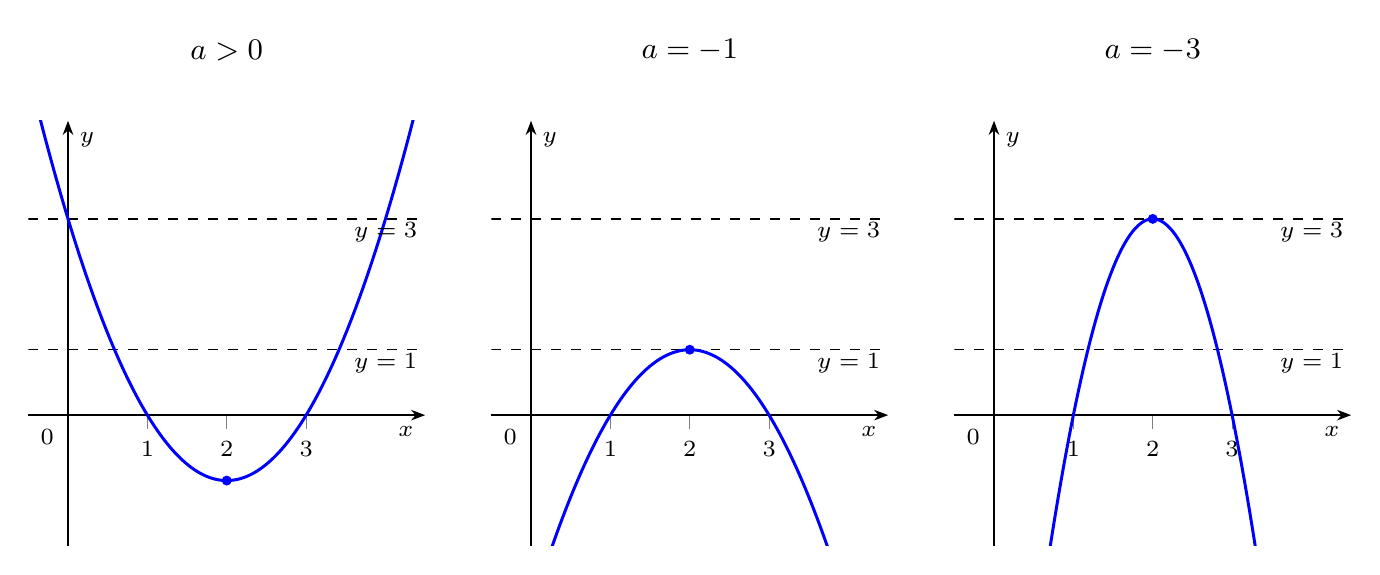
\begin{tikzpicture}[scale=1.2]
\pgfplotsset{
    solution panel/.style={
        width=4.2cm,height=4.5cm,
        scale only axis,
        xmin=-0.5,xmax=4.5,
        ymin=-2,ymax=4.5,
        axis lines=middle,
        axis line style={thin,black,-{Stealth[length=1.5mm]}},
        xtick={1,2,3},
        ytick=\empty,
        tick align=outside,
        font=\scriptsize,
        xlabel={$x$},
        ylabel={$y$},
        xlabel style={at={(axis cs:4.5,0)},anchor=north east},
        ylabel style={at={(axis cs:0,4.5)},anchor=north west},
        title style={font=\small,yshift=3mm},
        clip=true,
        clip mode=individual
    }
}

\begin{axis}[
    solution panel,
    at={(0cm,0cm)},anchor=south west,
    title={$a>0$}
]
\addplot[thin,black,dashed,domain=-0.5:4.5,samples=2] {1};
\addplot[thin,black,dashed,domain=-0.5:4.5,samples=2] {3};
\addplot[blue,line width=0.9pt,domain=-0.5:4.5,samples=161]
    {(x-2)^2-1};
\fill[blue] (axis cs:2,-1) circle[radius=1.5pt];
\node[below left=1pt] at (axis cs:0,0) {$0$};
\node[anchor=north east,inner sep=1pt]
    at (axis cs:4.45,1) {$y=1$};
\node[anchor=north east,inner sep=1pt]
    at (axis cs:4.45,3) {$y=3$};
\end{axis}

\begin{axis}[
    solution panel,
    at={(4.9cm,0cm)},anchor=south west,
    title={$a=-1$}
]
\addplot[thin,black,dashed,domain=-0.5:4.5,samples=2] {1};
\addplot[thin,black,dashed,domain=-0.5:4.5,samples=2] {3};
\addplot[blue,line width=0.9pt,domain=-0.5:4.5,samples=161]
    {1-(x-2)^2};
\fill[blue] (axis cs:2,1) circle[radius=1.5pt];
\node[below left=1pt] at (axis cs:0,0) {$0$};
\node[anchor=north east,inner sep=1pt]
    at (axis cs:4.45,1) {$y=1$};
\node[anchor=north east,inner sep=1pt]
    at (axis cs:4.45,3) {$y=3$};
\end{axis}

\begin{axis}[
    solution panel,
    at={(9.8cm,0cm)},anchor=south west,
    title={$a=-3$}
]
\addplot[thin,black,dashed,domain=-0.5:4.5,samples=2] {1};
\addplot[thin,black,dashed,domain=-0.5:4.5,samples=2] {3};
\addplot[blue,line width=0.9pt,domain=-0.5:4.5,samples=161]
    {3-3*(x-2)^2};
\fill[blue] (axis cs:2,3) circle[radius=1.5pt];
\node[below left=1pt] at (axis cs:0,0) {$0$};
\node[anchor=north east,inner sep=1pt]
    at (axis cs:4.45,1) {$y=1$};
\node[anchor=north east,inner sep=1pt]
    at (axis cs:4.45,3) {$y=3$};
\end{axis}

\end{tikzpicture}
% end q000777 figure F1
\end{djsSolutionFigure}

If $a>0$, the vertex lies below the $x$-axis, so both horizontal lines cut the parabola twice. This gives four solutions.

If $a<0$, the vertex is a maximum. A vertex at height $1$ gives only one solution: $y=1$ touches once and $y=3$ misses the curve. A vertex at height $3$ gives exactly three: $y=3$ touches once and $y=1$ cuts twice.

Therefore
\[
-a=3\implies a=-3
\]
and hence
\[
f(0)=-3(0-1)(0-3)=-9
\]

The correct option is \textbf{A}.\\[5pt]

\textit{Alternative Solution:}

Using $f(x)=a(x-1)(x-3)$, the equations $f(x)=1$ and $f(x)=3$ become
\[
\begin{aligned}
ax^2-4ax+3a-1&=0\\[5pt]
ax^2-4ax+3a-3&=0
\end{aligned}
\]

Their solution sets are disjoint. To give three distinct real solutions, one quadratic must have discriminant zero and the other must have positive discriminant.

Using $b^2-4ac$, their respective discriminants are
\[
\begin{aligned}
\Delta_1&=(-4a)^2-4a(3a-1)=4a(a+1)\\[5pt]
\Delta_3&=(-4a)^2-4a(3a-3)=4a(a+3)
\end{aligned}
\]

Since $a\ne0$, the two possibilities are
\[
\begin{aligned}
\Delta_1=0&\implies a=-1\implies \Delta_3=-8<0\\[5pt]
\Delta_3=0&\implies a=-3\implies \Delta_1=24>0
\end{aligned}
\]

Only $a=-3$ gives one repeated root and two further distinct real roots. Thus
\[
f(0)=-3(0-1)(0-3)=-9
\]

The correct option is \textbf{A}.
% end q000777 solution
\end{djsSolution}
\end{enumerate}
\clearpage
\thispagestyle{djssolutions}
\vspace*{8pt}
\djsTopicLine{Trigonometry}
\begin{enumerate}[label=\textbf{\arabic*.},leftmargin=*,itemsep=0pt,start=17]
\questionitem[Trigonometry]
% begin q000719 stem
A triangle has an angle of $120^\circ$ 

The perimeter of the triangle is $15$, and its area is $\dfrac{15\sqrt{3}}{4}$ \vspace*{5pt}

What is the length of the longest side of the triangle?
% end q000719 stem

\par\vspace*{12pt}
\begin{tabularx}{\linewidth}{@{}>{\bfseries}l Y@{}}
A &
% begin q000719 choice A
$5$
% end q000719 choice A
\\[0.8em]
B &
% begin q000719 choice B
$\dfrac{11}{2}$
% end q000719 choice B
\\[0.8em]
C &
% begin q000719 choice C
$6$
% end q000719 choice C
\\[0.8em]
D &
% begin q000719 choice D
$\dfrac{13}{2}$
% end q000719 choice D
\\[0.8em]
E &
% begin q000719 choice E
$7$
% end q000719 choice E
\\[0.8em]
F &
% begin q000719 choice F
$\dfrac{15}{2}$
% end q000719 choice F
\\[0.8em]
G &
% begin q000719 choice G
$8$
% end q000719 choice G
\\
\end{tabularx}

\begin{djsSolution}{E}
% begin q000719 solution
Let the sides adjacent to the $120^\circ$ angle be $a$ and $b$, and let the opposite side be $c$.

\begin{djsSolutionFigure}
% begin q000719 figure F1
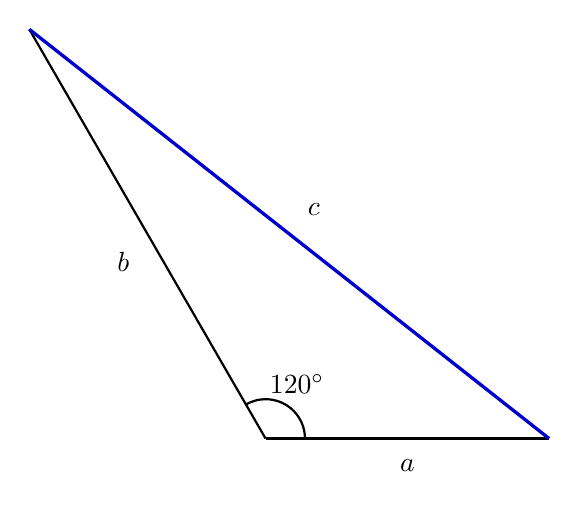
\begin{tikzpicture}[scale=1.2]
\coordinate (P) at (0,0);
\coordinate (Q) at (3,0);
\coordinate (R) at ({-5/2},{5*sqrt(3)/2});

\draw[thick,black] (P) -- (Q)
    node[midway,below=4pt] {$a$};
\draw[thick,black] (P) -- (R)
    node[midway,below left=4pt] {$b$};
\draw[very thick,blue!80!black] (Q) -- (R)
    node[midway,above right=4pt,text=black] {$c$};

\pic[draw,thick,"$120^\circ$",angle radius=5mm,angle eccentricity=1.6]
    {angle=Q--P--R};
\end{tikzpicture}
% end q000719 figure F1
\end{djsSolutionFigure}

The other two angles sum to $60^\circ$, so $120^\circ$ is the largest angle. The longest side is opposite the largest angle, so we need to find $c$.

Using the area formula $\text{area}=\frac12 ab\sin\theta$ and $\sin120^\circ=\frac{\sqrt3}{2}$,
\[
\frac12 ab\sin120^\circ
=\frac{ab\sqrt3}{4} = \frac{15\sqrt3}{4}
\implies ab=15
\]

The perimeter gives
\[
a+b+c=15 \implies a+b=15-c
\]

By the cosine rule, with $\cos120^\circ=-\frac12$,
\begin{align*}
    c^2&=a^2+b^2-2ab\cos120^\circ\\[5pt]
&=a^2+b^2+ab
\end{align*}

We know $a+b$ and $ab$, rather than $a$ and $b$ separately, so use
$a^2+b^2=(a+b)^2-2ab$. Substituting $a+b=15-c$ and $ab=15$ gives
\[
c^2=(15-c)^2-15
\]
Expanding and cancelling $c^2$ from both sides,
\[
\begin{aligned}
c^2&=225-30c+c^2-15\\[5pt]
0&=210-30c
\end{aligned}
\]

Hence
\[
30c=210 \implies c=7
\]
This also satisfies the triangle inequality for the longest side, since $c=7<8=a+b$.

Thus the longest side has length $7$, and the correct option is \textbf{E}.
% end q000719 solution
\end{djsSolution}
\end{enumerate}
\clearpage
\thispagestyle{djssolutions}
\vspace*{8pt}
\djsTopicLine{Coordinate Geometry}
\begin{enumerate}[label=\textbf{\arabic*.},leftmargin=*,itemsep=0pt,start=18]
\questionitem[Coordinate Geometry]
% begin q000653 stem
The point $A$ has coordinates $(-7,-5)$ and the point $B$ has coordinates $(23,45)$.

How many points on the straight line segment $AB$ have both coordinates equal to integers, not counting $A$ and $B$ themselves?
% end q000653 stem

\par\vspace*{12pt}
\begin{tabularx}{\linewidth}{@{}>{\bfseries}l Y@{}}
A &
% begin q000653 choice A
$4$
% end q000653 choice A
\\[0.8em]
B &
% begin q000653 choice B
$5$
% end q000653 choice B
\\[0.8em]
C &
% begin q000653 choice C
$9$
% end q000653 choice C
\\[0.8em]
D &
% begin q000653 choice D
$10$
% end q000653 choice D
\\[0.8em]
E &
% begin q000653 choice E
$11$
% end q000653 choice E
\\[0.8em]
F &
% begin q000653 choice F
$29$
% end q000653 choice F
\\[0.8em]
G &
% begin q000653 choice G
$49$
% end q000653 choice G
\\
\end{tabularx}

\begin{djsSolution}{C}
% begin q000653 solution
The horizontal and vertical changes from $A$ to $B$ are
\[
23-(-7)=30
\qquad\text{and}\qquad
45-(-5)=50
\]

\begin{djsSolutionFigure}
% begin q000653 figure F1
\begin{tikzpicture}
\coordinate (A) at (0,0);
\coordinate (B) at (4,6.7);
\coordinate (C) at (4,0);

\draw[thin,dashed,black] (A) -- (C)
    node[midway,below=4pt] {$30$};
\draw[thin,dashed,black] (C) -- (B)
    node[midway,right=4pt] {$50$};
\draw[very thick,blue] (A) -- (B);

\node[left=4pt] at (A) {$A\,(-7,-5)$};
\node[above=4pt] at (B) {$B\,(23,45)$};
\end{tikzpicture}
% end q000653 figure F1
\end{djsSolutionFigure}

Since $30:50=3:5$, each step $\begin{pmatrix}3\\5\end{pmatrix}$ takes us from one integer-coordinate point to another on the line.

To see that these steps miss no such points, the line equation $y-y_1=m(x-x_1)$ gives
\[
y+5=\frac53(x+7)
\implies 3(y+5)=5(x+7)
\]

If $x$ and $y$ are integers, $5(x+7)$ must be divisible by $3$. Since $3$ and $5$ have no common factor, $x+7=3k$ for some integer $k$. The line equation then gives
\[
y+5=\frac53(3k)=5k
\]

Hence every integer-coordinate point on the line has the form
\[
\begin{pmatrix}x\\y\end{pmatrix}
=
\begin{pmatrix}-7\\-5\end{pmatrix}
+k\begin{pmatrix}3\\5\end{pmatrix}
\]
so it lies a whole number of these steps from $A$.

Now
\[
\overrightarrow{AB}
=\begin{pmatrix}30\\50\end{pmatrix}
=10\begin{pmatrix}3\\5\end{pmatrix}
\]
so $A$ corresponds to $k=0$ and $B$ to $k=10$. The interior points therefore correspond to $k=1,2,\ldots,9$, giving $\boxed{9}$ points.

The correct option is \textbf{C}.
% end q000653 solution
\end{djsSolution}
\end{enumerate}
\clearpage
\thispagestyle{djssolutions}
\vspace*{8pt}
\djsTopicLine{Algebra}
\begin{enumerate}[label=\textbf{\arabic*.},leftmargin=*,itemsep=0pt,start=19]
\questionitem[Algebra]
% begin q000751 stem
The positive real numbers $x$ and $y$ satisfy the equations
\[x\sqrt{y} + y\sqrt{x} = 8\]
and
\[x\sqrt{x} + y\sqrt{y} = 40\]
What is the value of $x + y$?
% end q000751 stem

\par\vspace*{12pt}
\begin{tabularx}{\linewidth}{@{}>{\bfseries}l Y@{}}
A &
% begin q000751 choice A
$6$
% end q000751 choice A
\\[0.8em]
B &
% begin q000751 choice B
$8$
% end q000751 choice B
\\[0.8em]
C &
% begin q000751 choice C
$10$
% end q000751 choice C
\\[0.8em]
D &
% begin q000751 choice D
$12$
% end q000751 choice D
\\[0.8em]
E &
% begin q000751 choice E
$14$
% end q000751 choice E
\\[0.8em]
F &
% begin q000751 choice F
$16$
% end q000751 choice F
\\
\end{tabularx}

\begin{djsSolution}{D}
% begin q000751 solution
The square roots suggest the substitution
\[
a=\sqrt{x},\qquad b=\sqrt{y}
\]
where $a$ and $b$ are positive. Then $x=a^2$ and $y=b^2$, so the given equations become
\[
\begin{aligned}
a^2b+ab^2&=8\\[5pt]
a^3+b^3&=40
\end{aligned}
\]

Factorising the first equation gives
\[
ab(a+b)=8
\]

To find $a+b$, expand its cube directly:
\[
\begin{aligned}
(a+b)^3
&=(a^2+2ab+b^2)(a+b)\\[5pt]
&=a^3+3a^2b+3ab^2+b^3\\[5pt]
&=(a^3+b^3)+3(a^2b+ab^2)
\end{aligned}
\]

This expansion combines the second given equation with three times the first. Substituting their values gives
\[
(a+b)^3=40+3(8)=64
\]

Taking the cube root,
\[
\boxed{a+b=4}
\]

Substituting into the factored first equation,
\[
4ab=8
\]

Dividing by $4$,
\[
\boxed{ab=2}
\]

We do not need to find $a$ and $b$ separately, because expanding the square of their sum gives
\[
(a+b)^2=a^2+2ab+b^2
\]

Rearranging and substituting,
\[
\begin{aligned}
a^2+b^2&=(a+b)^2-2ab\\[5pt]
&=4^2-2(2)\\[5pt]
&=12
\end{aligned}
\]

Therefore
\[
x+y=12
\]

The correct option is \textbf{D}.\\[5pt]

\textit{Remark:} 

We could instead use $a+b=4$ and $ab=2$ to find $a$ and $b$ separately:
\[
a(4-a)=2
\implies a^2-4a+2=0
\implies a=2\pm\sqrt2
\]
Then $b=4-a$ is the other value, so
\[
x+y=(2+\sqrt2)^2+(2-\sqrt2)^2=12
\]
This works, but finding $a$ and $b$ individually is unnecessary. 
% end q000751 solution
\end{djsSolution}
\end{enumerate}
\clearpage
\thispagestyle{djssolutions}
\vspace*{8pt}
\djsTopicLine{Integration}
\begin{enumerate}[label=\textbf{\arabic*.},leftmargin=*,itemsep=0pt,start=20]
\questionitem[Integration]
% begin q000729 stem
Let $f$ be a polynomial of degree at most $3$ with real coefficients.

For $t>0$, define
\[
D(t)=\int_0^t f(x)\,\mathrm{d}x-\int_{-t}^0 f(x)\,\mathrm{d}x
\]
Which of the following statements are true?
\[
\begin{array}{@{}ll@{}}
\textbf{I} & \text{If }f(x)=f(-x)\text{ for every real }x,\text{ then }D(1)=0 \\[5pt]
\textbf{II} & \text{If }D(1)=0,\text{ then }f(x)=f(-x)\text{ for every real }x \\[5pt]
\textbf{III} & \text{If }D(1)=D(2)=0,\text{ then }f(x)=f(-x)\text{ for every real }x \\[5pt]
\end{array}
\]
% end q000729 stem

\par\vspace*{12pt}
\begin{tabularx}{\linewidth}{@{}>{\bfseries}l Y@{}}
A &
% begin q000729 choice A
None of them
% end q000729 choice A
\\[0.8em]
B &
% begin q000729 choice B
I only
% end q000729 choice B
\\[0.8em]
C &
% begin q000729 choice C
II only
% end q000729 choice C
\\[0.8em]
D &
% begin q000729 choice D
III only
% end q000729 choice D
\\[0.8em]
E &
% begin q000729 choice E
I and II only
% end q000729 choice E
\\[0.8em]
F &
% begin q000729 choice F
I and III only
% end q000729 choice F
\\[0.8em]
G &
% begin q000729 choice G
II and III only
% end q000729 choice G
\\[0.8em]
H &
% begin q000729 choice H
I, II and III
% end q000729 choice H
\\
\end{tabularx}

\begin{djsSolution}{F}
% begin q000729 solution
The condition $f(x)=f(-x)$ for every real $x$ is the definition of an \emph{even function}. Even functions are precisely those for which the $y$-axis is a line of symmetry.

A polynomial is an even function precisely when it contains only even powers of $x$. This includes the constant term, which we view as the $x^0$ term. To see this, write
\[
f(x)=ax^3+bx^2+cx+k
\]

where the coefficients may be zero, so this includes every polynomial of degree at most $3$.

Replacing $x$ by $-x$ gives
\[
f(-x)=-ax^3+bx^2-cx+k
\]

For this to equal $f(x)$ for every real $x$, corresponding coefficients must agree:
\[
a=-a,\qquad c=-c
\implies a=c=0
\]
Thus the condition is exactly that both odd-power coefficients vanish, as we expected for the definition of an even function applied to a cubic.

Now calculate the two integrals:
\[
\begin{aligned}
\int_0^t f(x)\,\mathrm{d}x
&=\left[\frac{ax^4}{4}+\frac{bx^3}{3}+\frac{cx^2}{2}+kx\right]_0^t\\[8pt]
&=\frac{at^4}{4}+\frac{bt^3}{3}+\frac{ct^2}{2}+kt
\end{aligned}
\]
and
\[
\begin{aligned}
\int_{-t}^0 f(x)\,\mathrm{d}x
&=\left[\frac{ax^4}{4}+\frac{bx^3}{3}+\frac{cx^2}{2}+kx\right]_{-t}^0\\[8pt]
&=0-\left(\frac{at^4}{4}-\frac{bt^3}{3}+\frac{ct^2}{2}-kt\right)\\[8pt]
&=-\frac{at^4}{4}+\frac{bt^3}{3}-\frac{ct^2}{2}+kt
\end{aligned}
\]

Subtracting, the contributions from $bx^2$ and $k$ cancel, giving
\[
\boxed{D(t)=\frac{1}{2}at^4+ct^2}
\]

\textbf{Statement I.} If $f(x)=f(-x)$ for every real $x$, then $a=c=0$ as discussed above. Hence
\[
D(1)=\frac02+0=0
\]
Statement I is true. \\

\textbf{Statement II.} The condition $D(1)=0$ gives
\[
\frac a2+c=0 \implies c=-\frac a2
\]
This relates the coefficients but does not force both to be zero. For example, take $f(x)=2x^3-x$. Then
\[
D(1)=\frac22-1=0
\]
but $f(1)=1$ and $f(-1)=-1$, so $f$ is not even. Statement II is false. \\

\textbf{Statement III.} The two conditions give
\[
\begin{aligned}
D(1)=0&\implies \frac a2+c=0\\[5pt]
D(2)=0&\implies 8a+4c=0
\end{aligned}
\]

From the first equation, $c=-\frac a2$. Substituting into the second,
\[
8a+4\left(-\frac a2\right)=0
\implies 6a=0
\implies a=0
\]
Then $c=-\frac a2=0$ as well. Both odd-power coefficients vanish, so $f(x)=f(-x)$ for every real $x$. Statement III is true.

Thus I and III only are true, so the correct option is \textbf{F}.
% end q000729 solution
\end{djsSolution}
\end{enumerate}
\end{document}
